\documentclass[12pt,a4paper]{ctexart}

\usepackage[margin=2.2cm]{geometry}
\usepackage{graphicx}
\usepackage{hyperref}
\usepackage{float}
\usepackage{caption}

\hypersetup{
  hidelinks
}

\setlength{\parskip}{0.45em}
\setlength{\parindent}{2em}
\graphicspath{{黑盒测试对话截图/}{白盒测试对话截图1/}{白盒测试2对话截图/}}

% 白盒截图占位：图片未放入时也可编译，并提示应放置内容
\newcommand{\recordfig}[3]{
  \begin{figure}[H]
    \centering
    \IfFileExists{#1}{
      \includegraphics[width=0.92\textwidth]{#1}
    }{
      \fbox{\parbox{0.88\textwidth}{
        \textbf{截图占位（待补充）}\\
        预期文件：\texttt{#1}\\
        建议内容：#3
      }}
    }
    \caption{#2}
  \end{figure}
}

\begin{document}

\begin{center}
{\LARGE\heiti 基于大模型的软件测试使用记录}
\end{center}

\section{黑盒测试使用记录}

\subsection{任务一：测试计划}

先向模型说明课程作业要求，并请模型判断当前应优先完成的任务。随后继续要求模型检查《黑盒测试计划》是否有多余内容，并按更贴合作业要求的方式调整文档结构。

\begin{figure}[H]
  \centering
  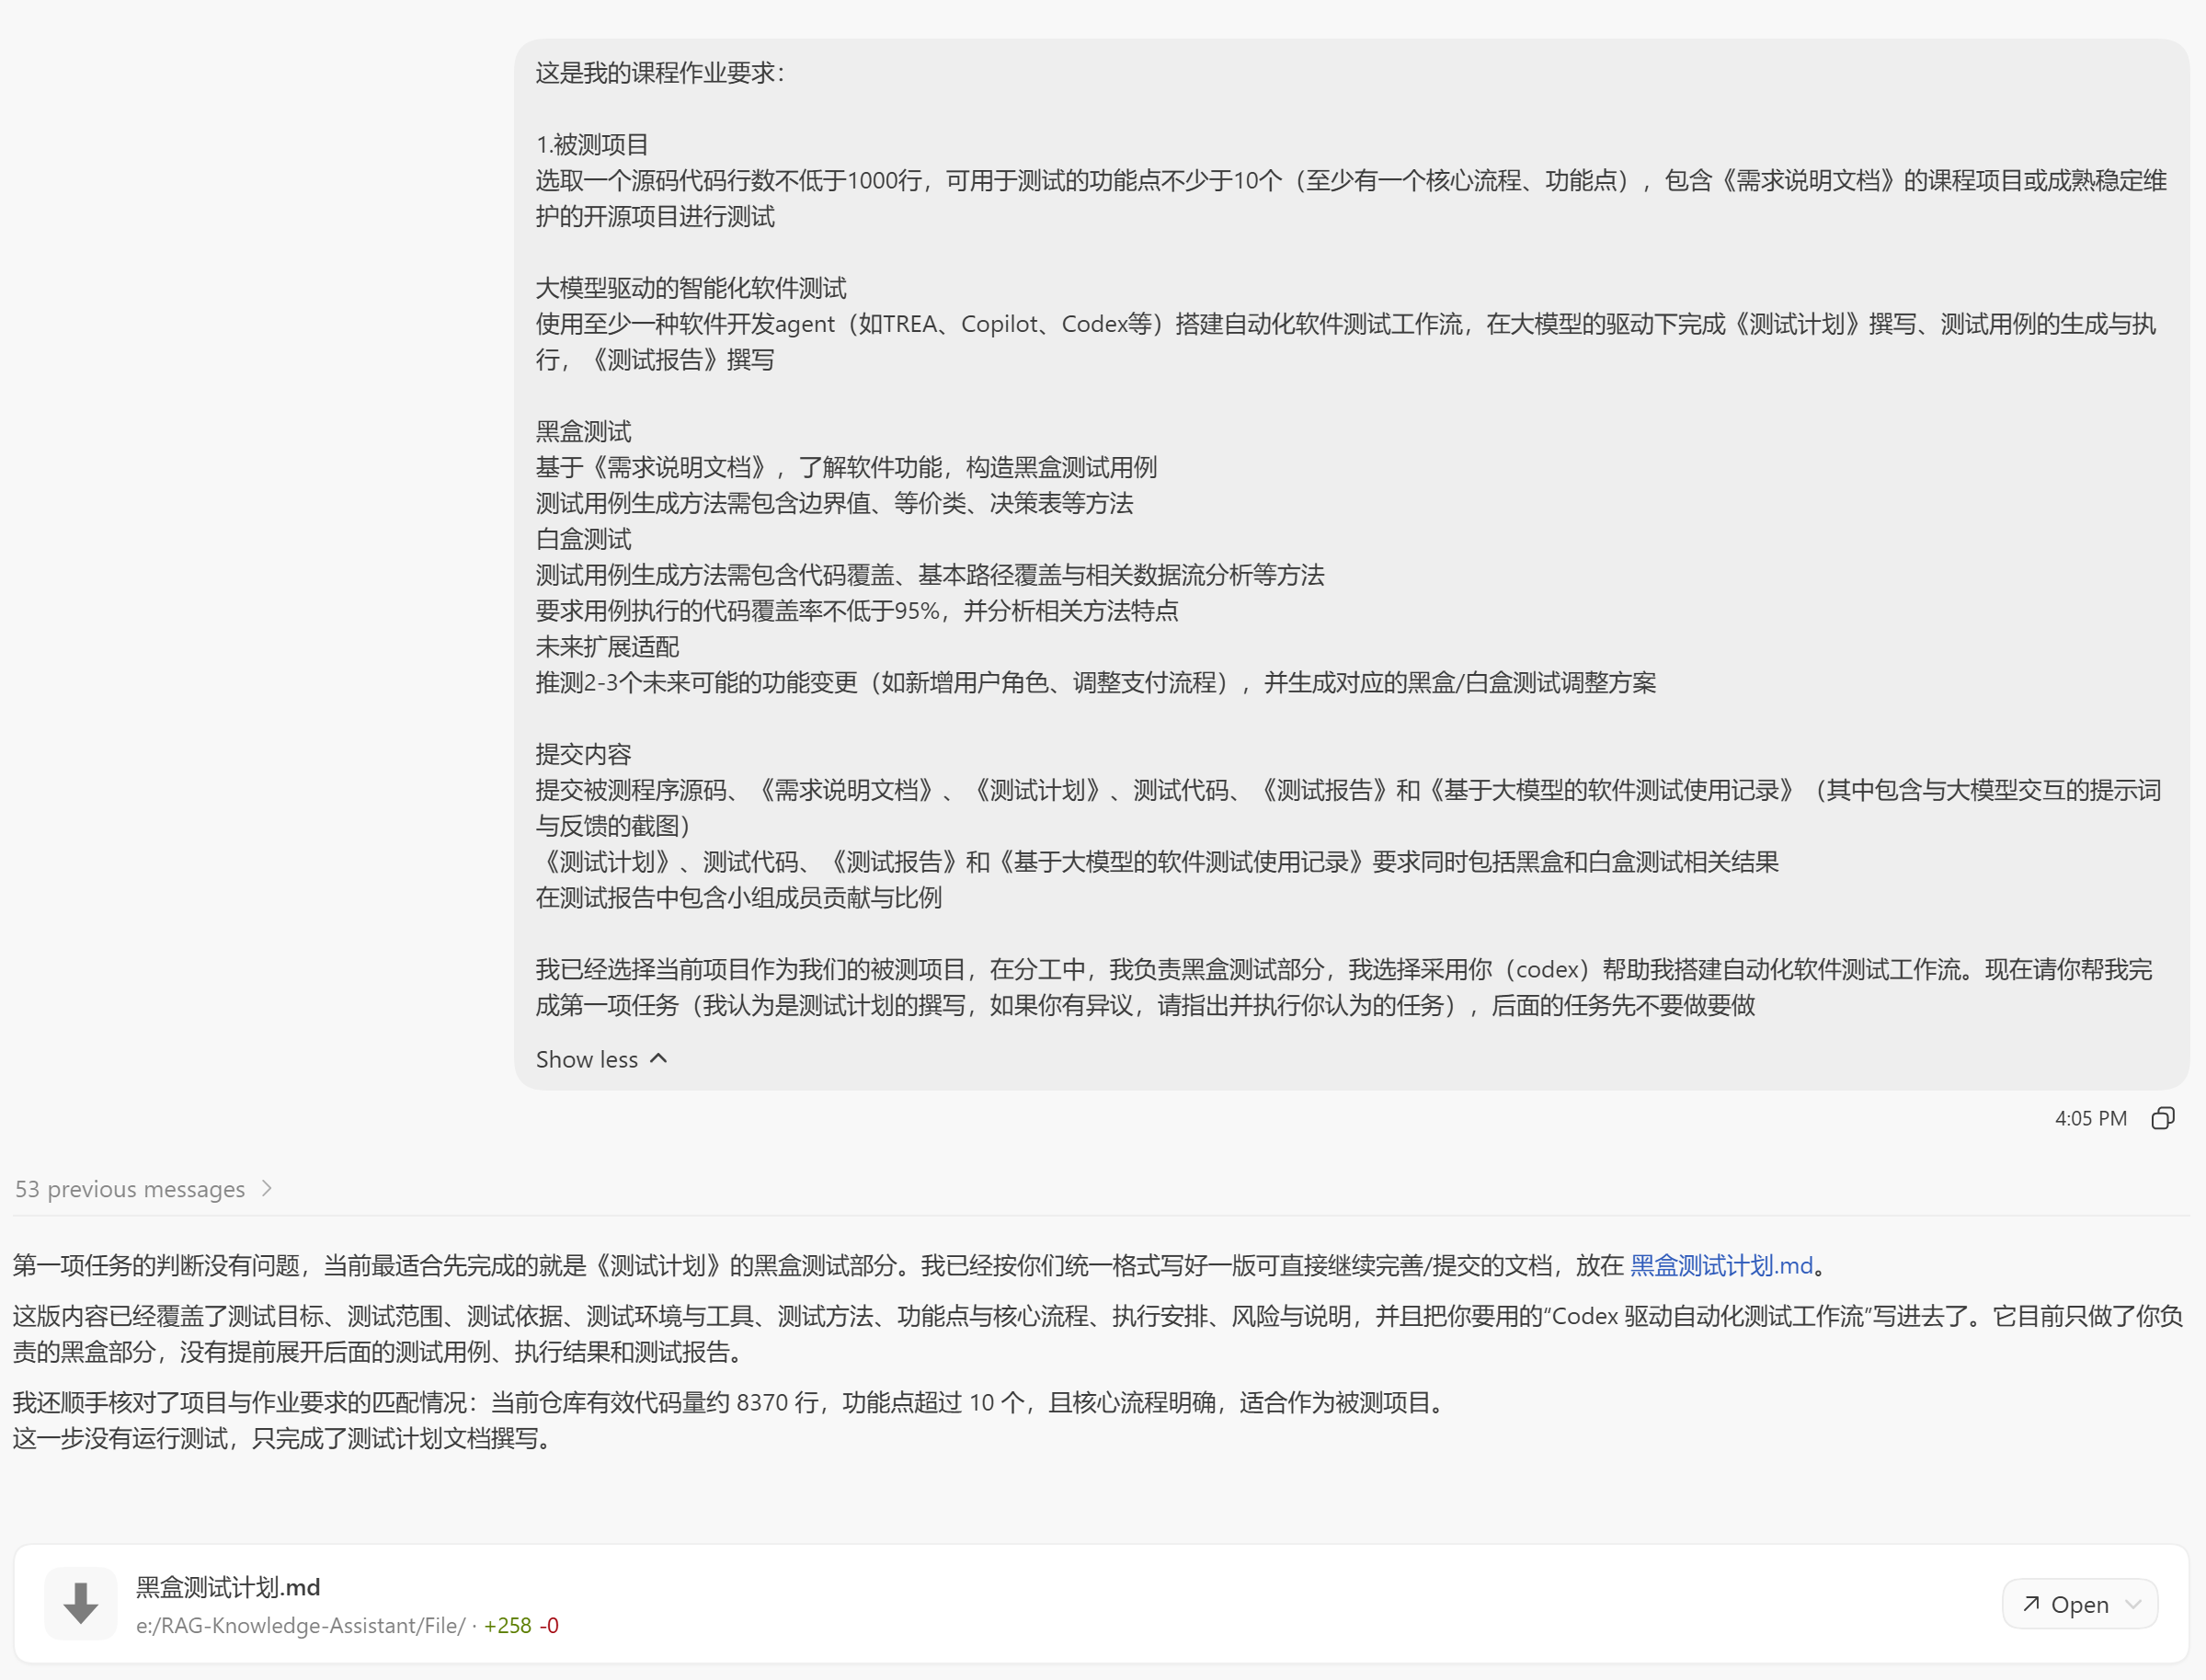
\includegraphics[width=0.92\textwidth]{任务1开始.png}
  \caption{任务一开始：提供课程作业要求，并请模型先完成黑盒测试计划}
\end{figure}

\begin{figure}[H]
  \centering
  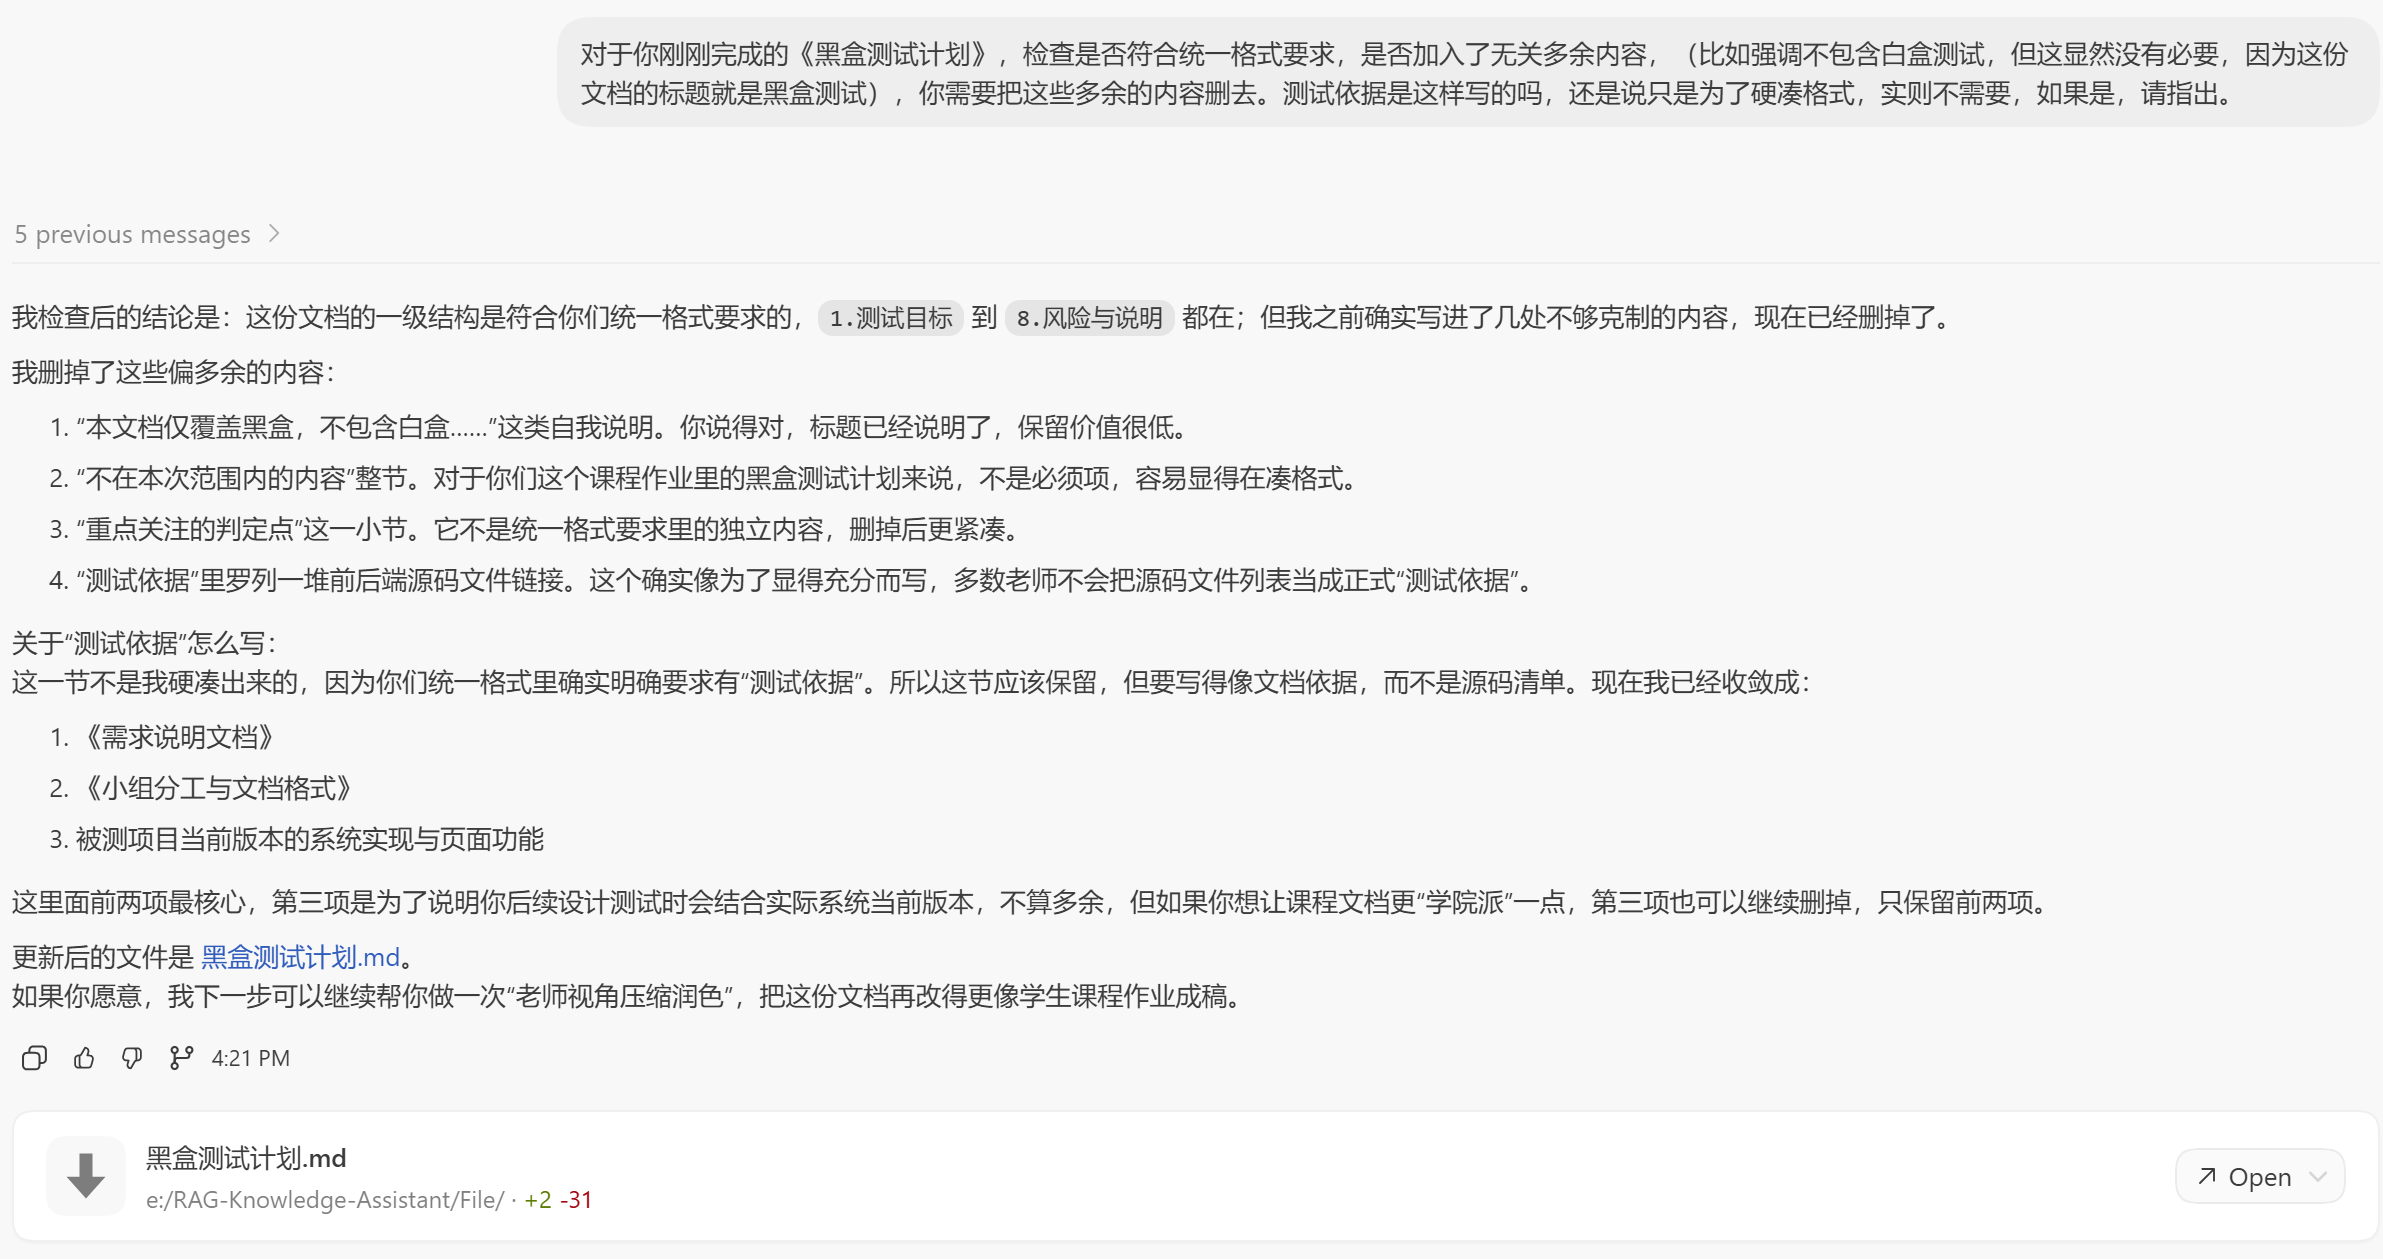
\includegraphics[width=0.92\textwidth]{任务1改进.png}
  \caption{任务一改进：继续检查测试计划是否存在多余内容并进行精简}
\end{figure}

\subsection{任务二：测试用例}

继续让模型完成黑盒测试用例设计。模型根据前面的任务顺序判断，继续生成黑盒测试用例，并说明已经覆盖用户、课程、资料、练习题、社区和核心流程等模块。

\begin{figure}[H]
  \centering
  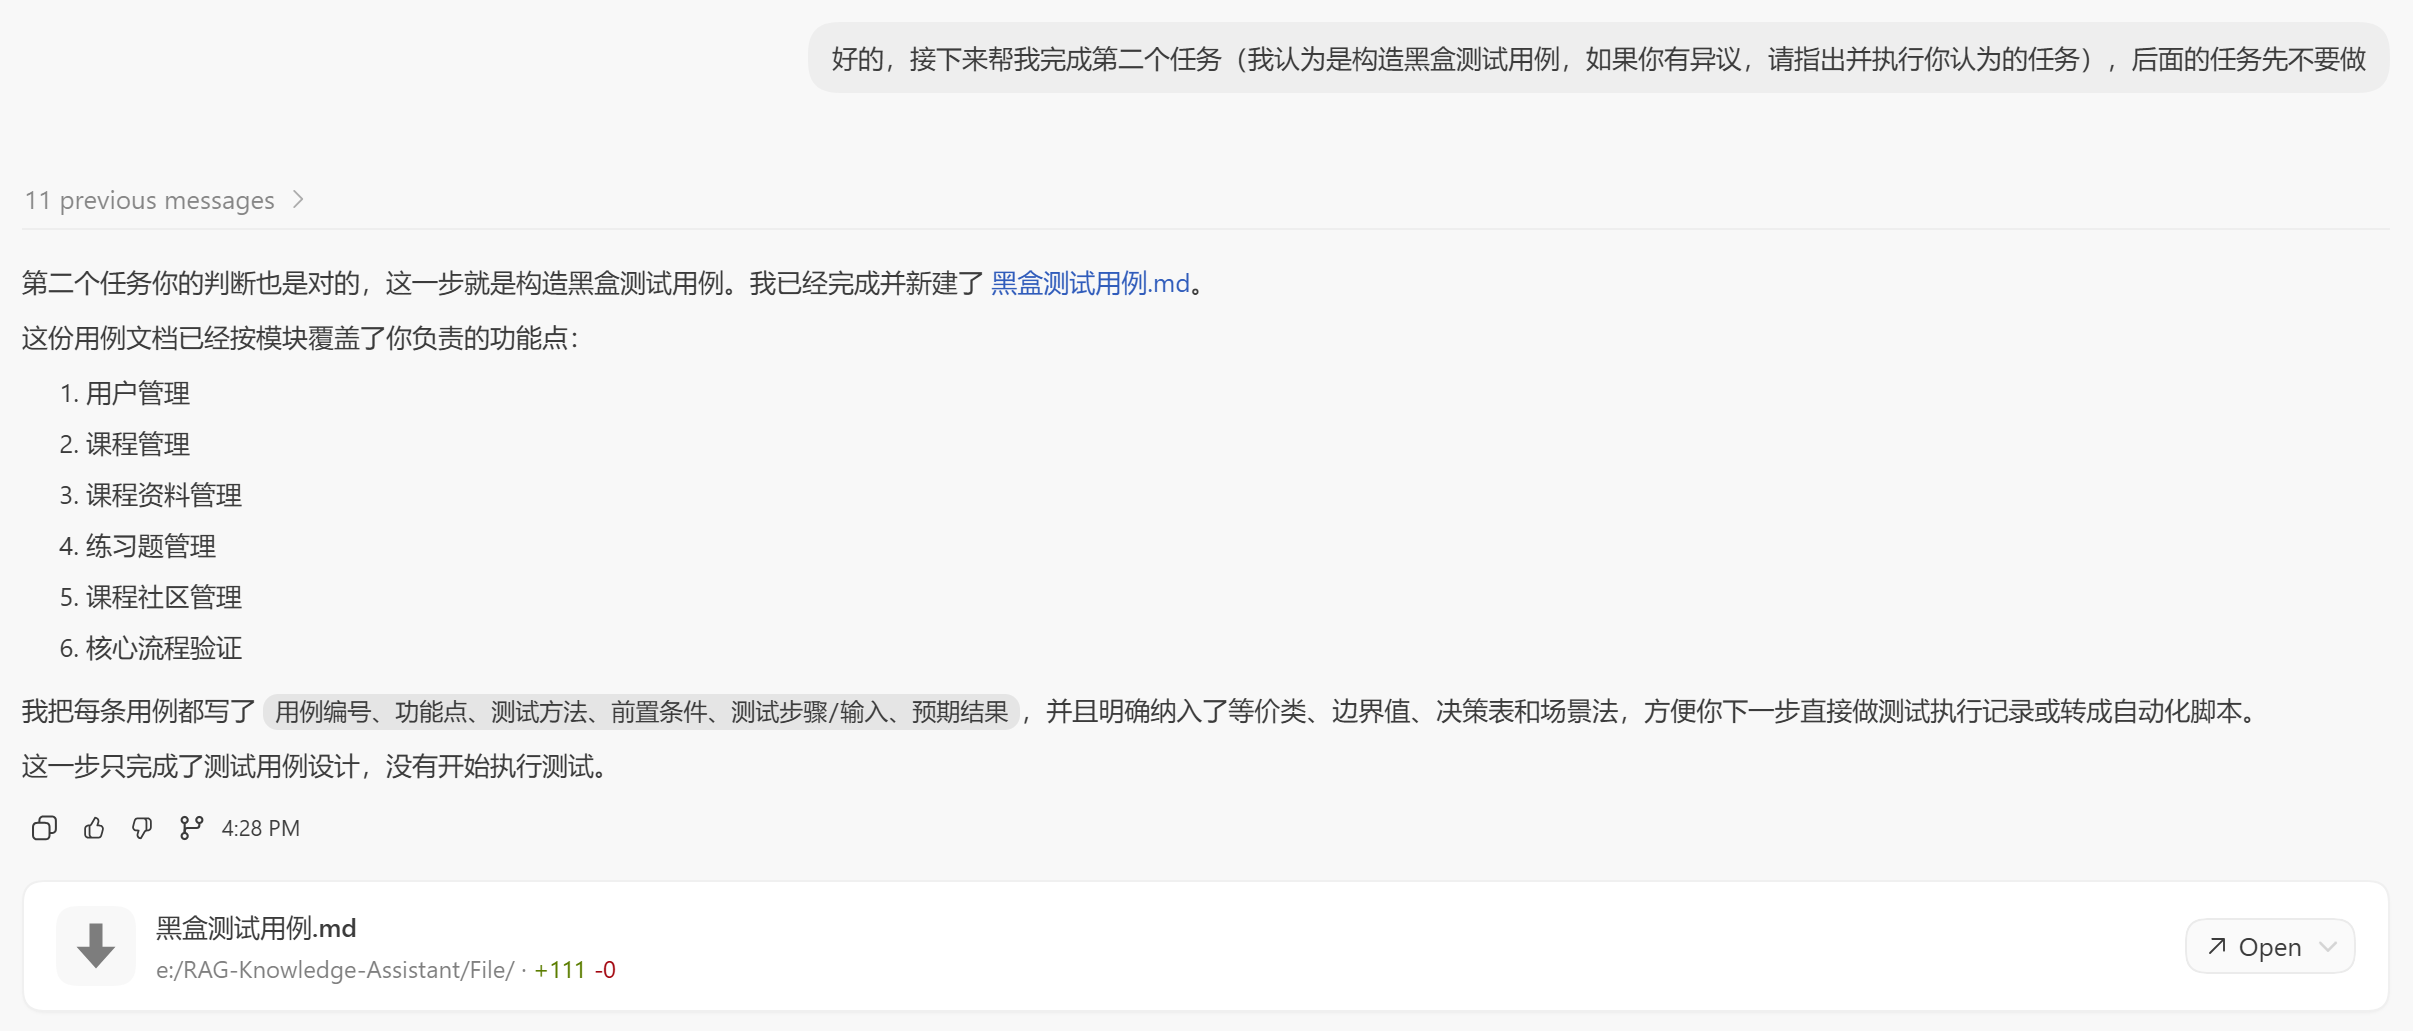
\includegraphics[width=0.92\textwidth]{任务2开始.png}
  \caption{任务二：构造黑盒测试用例}
\end{figure}

\subsection{任务三：生成并执行黑盒测试}

这一阶段主要涉及“第三项任务到底是什么”“是否要先写测试代码”“自动化测试是否偏离黑盒测试”“是否需要少量人工补充”等问题。从编写自动化测试代码，到执行测试，再到继续调整测试结构和说明黑盒边界，相关交互见下列截图。

\begin{figure}[H]
  \centering
  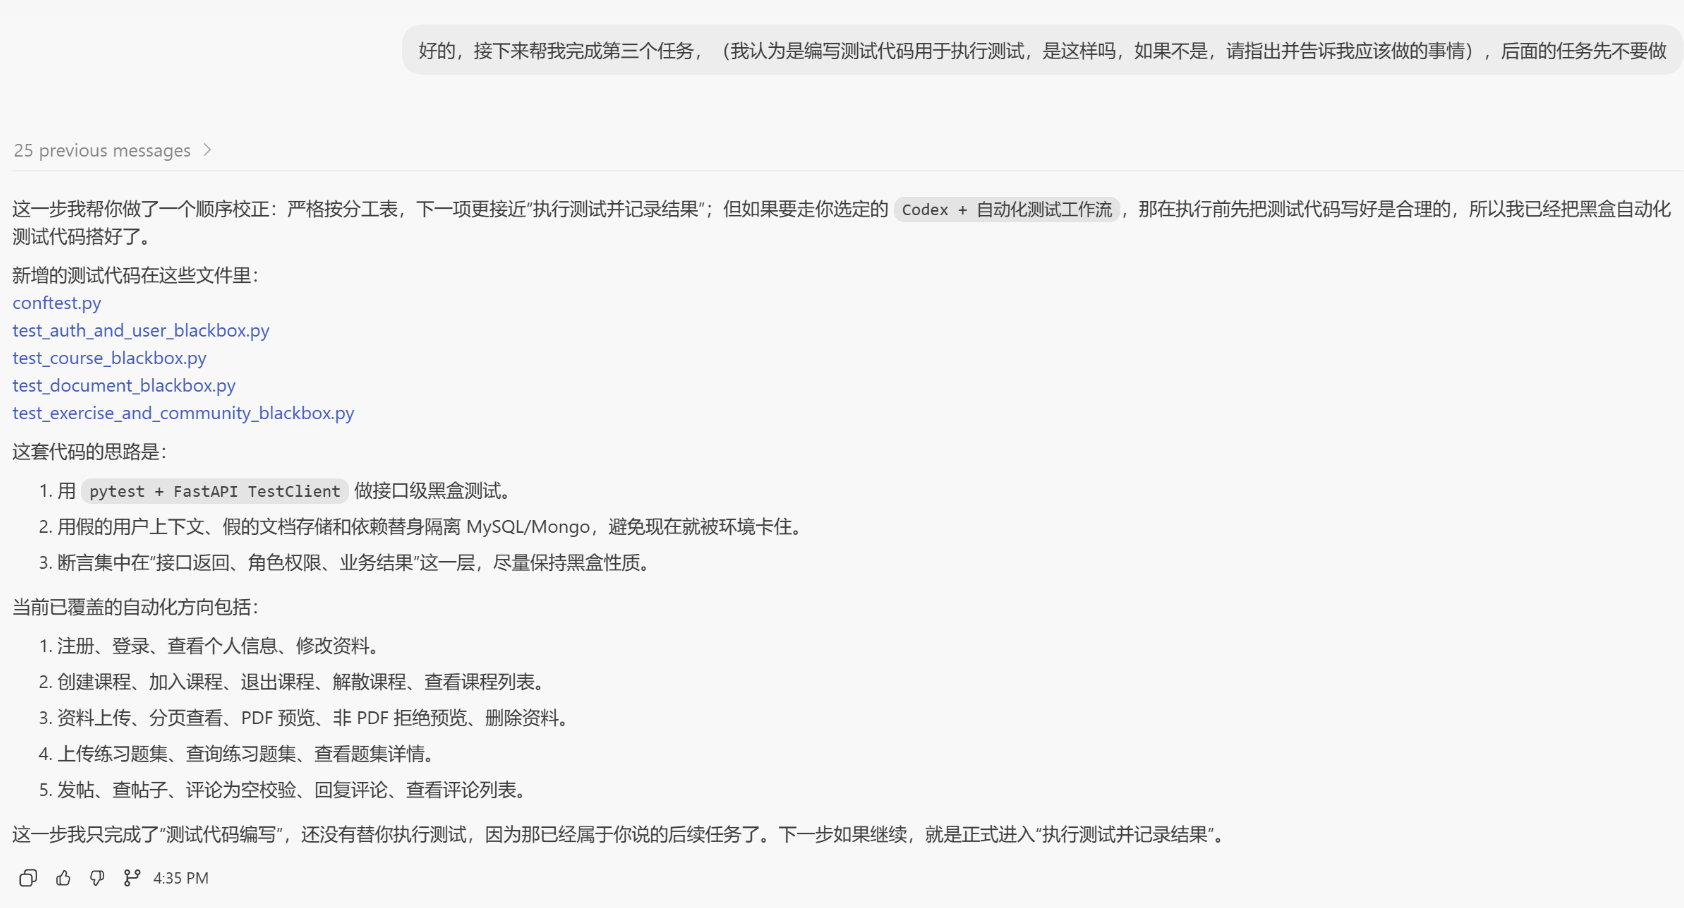
\includegraphics[width=0.92\textwidth]{任务3开始.png}
  \caption{任务三开始：初次确认第三项任务应围绕生成并执行黑盒测试展开}
\end{figure}

\begin{figure}[H]
  \centering
  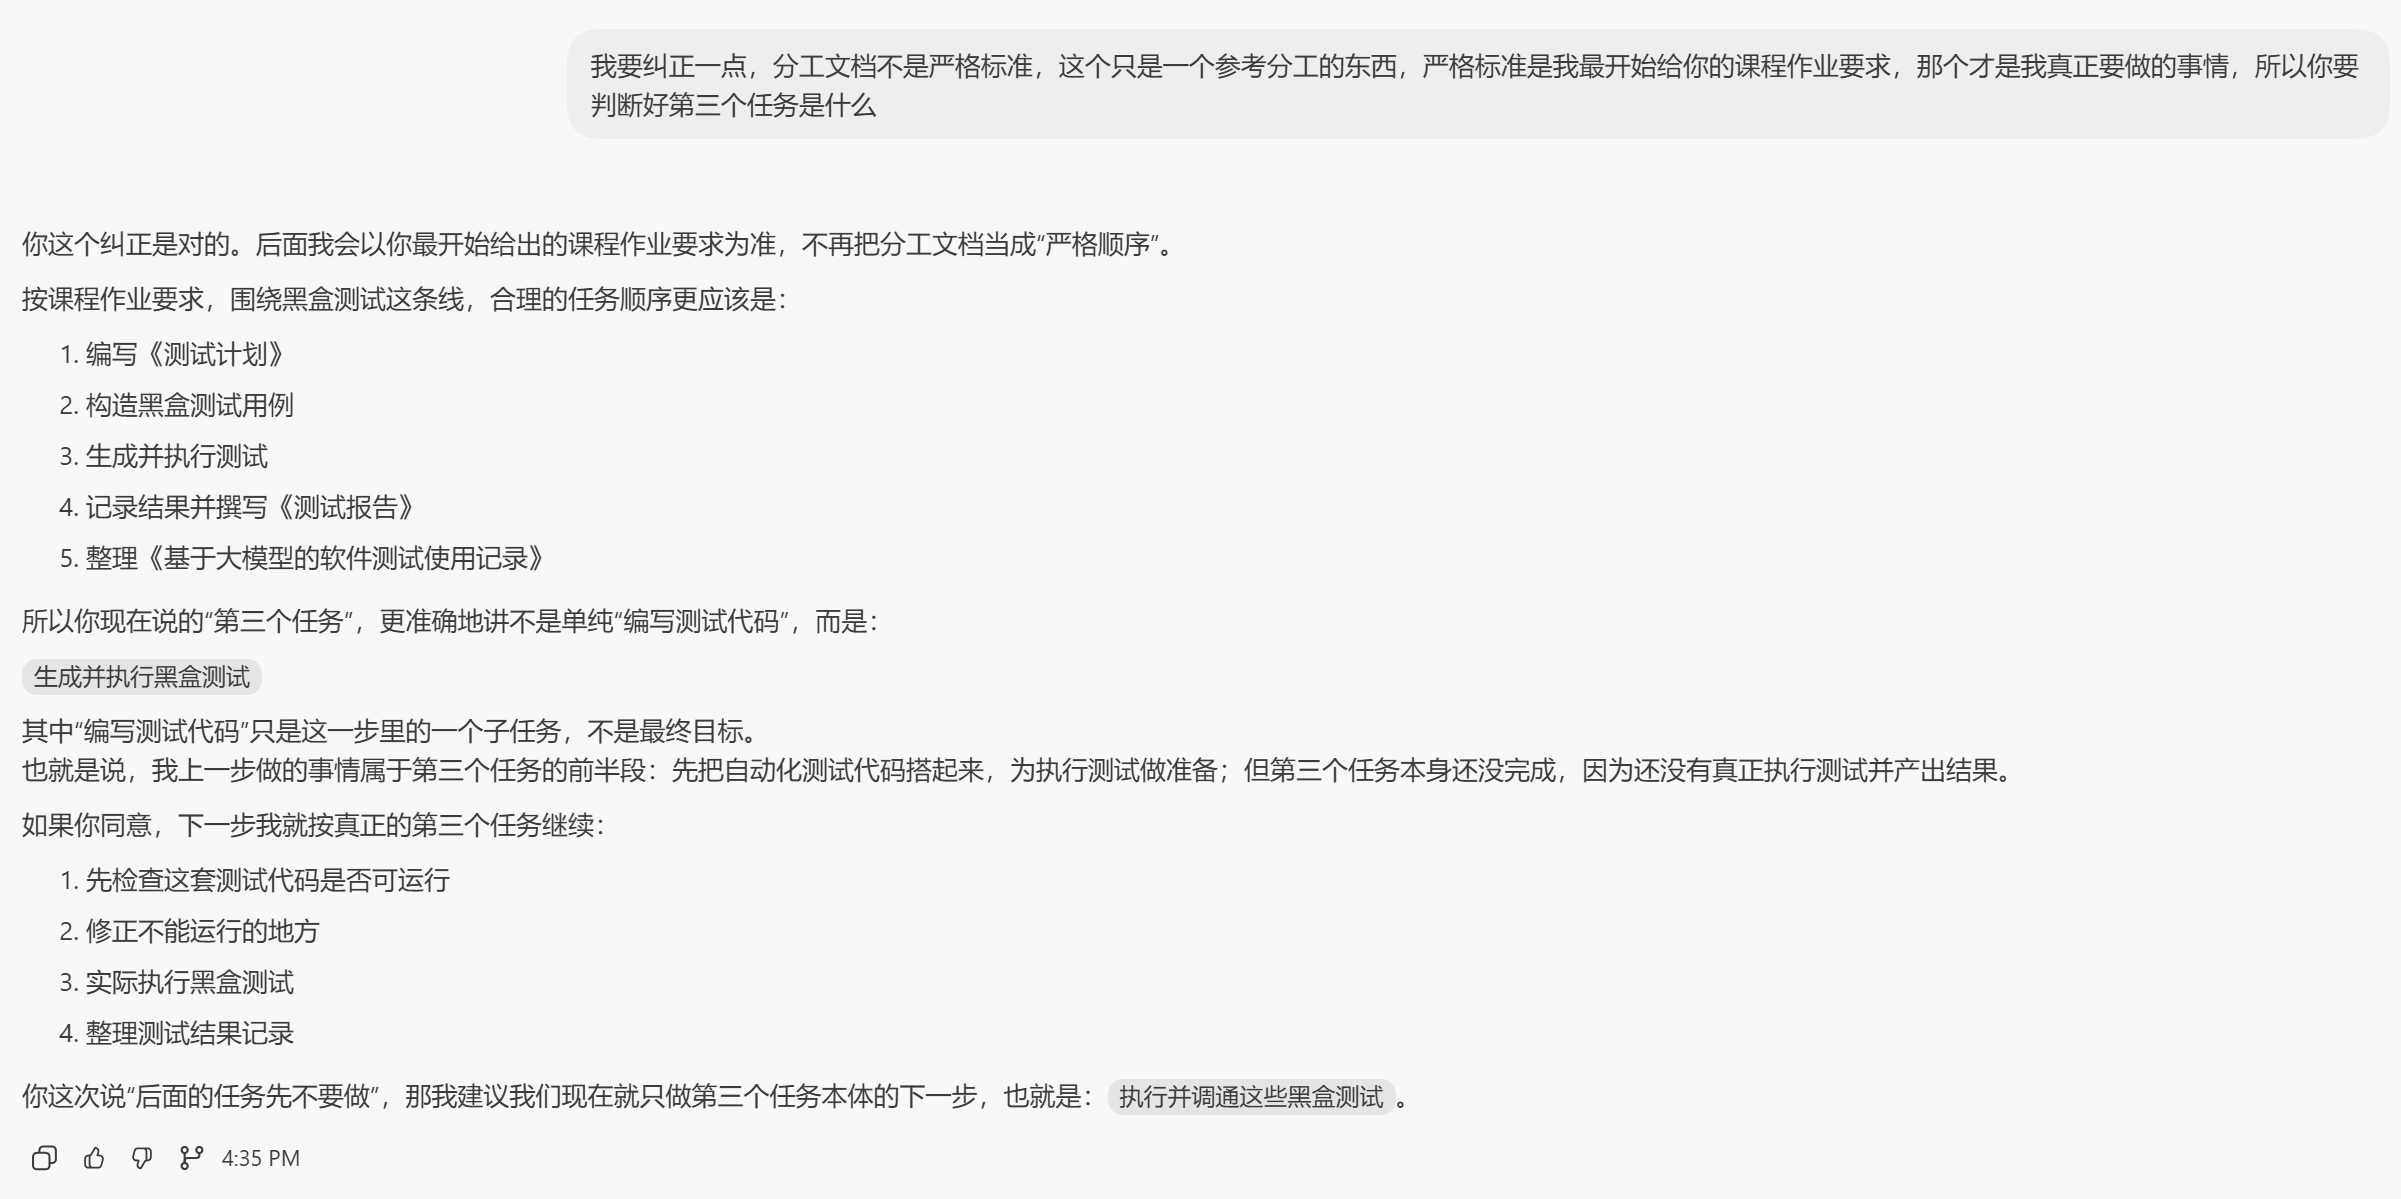
\includegraphics[width=0.92\textwidth]{任务3调整.png}
  \caption{任务三调整：围绕“测试代码为主、必要时少量人工”的要求调整测试方案}
\end{figure}

\begin{figure}[H]
  \centering
  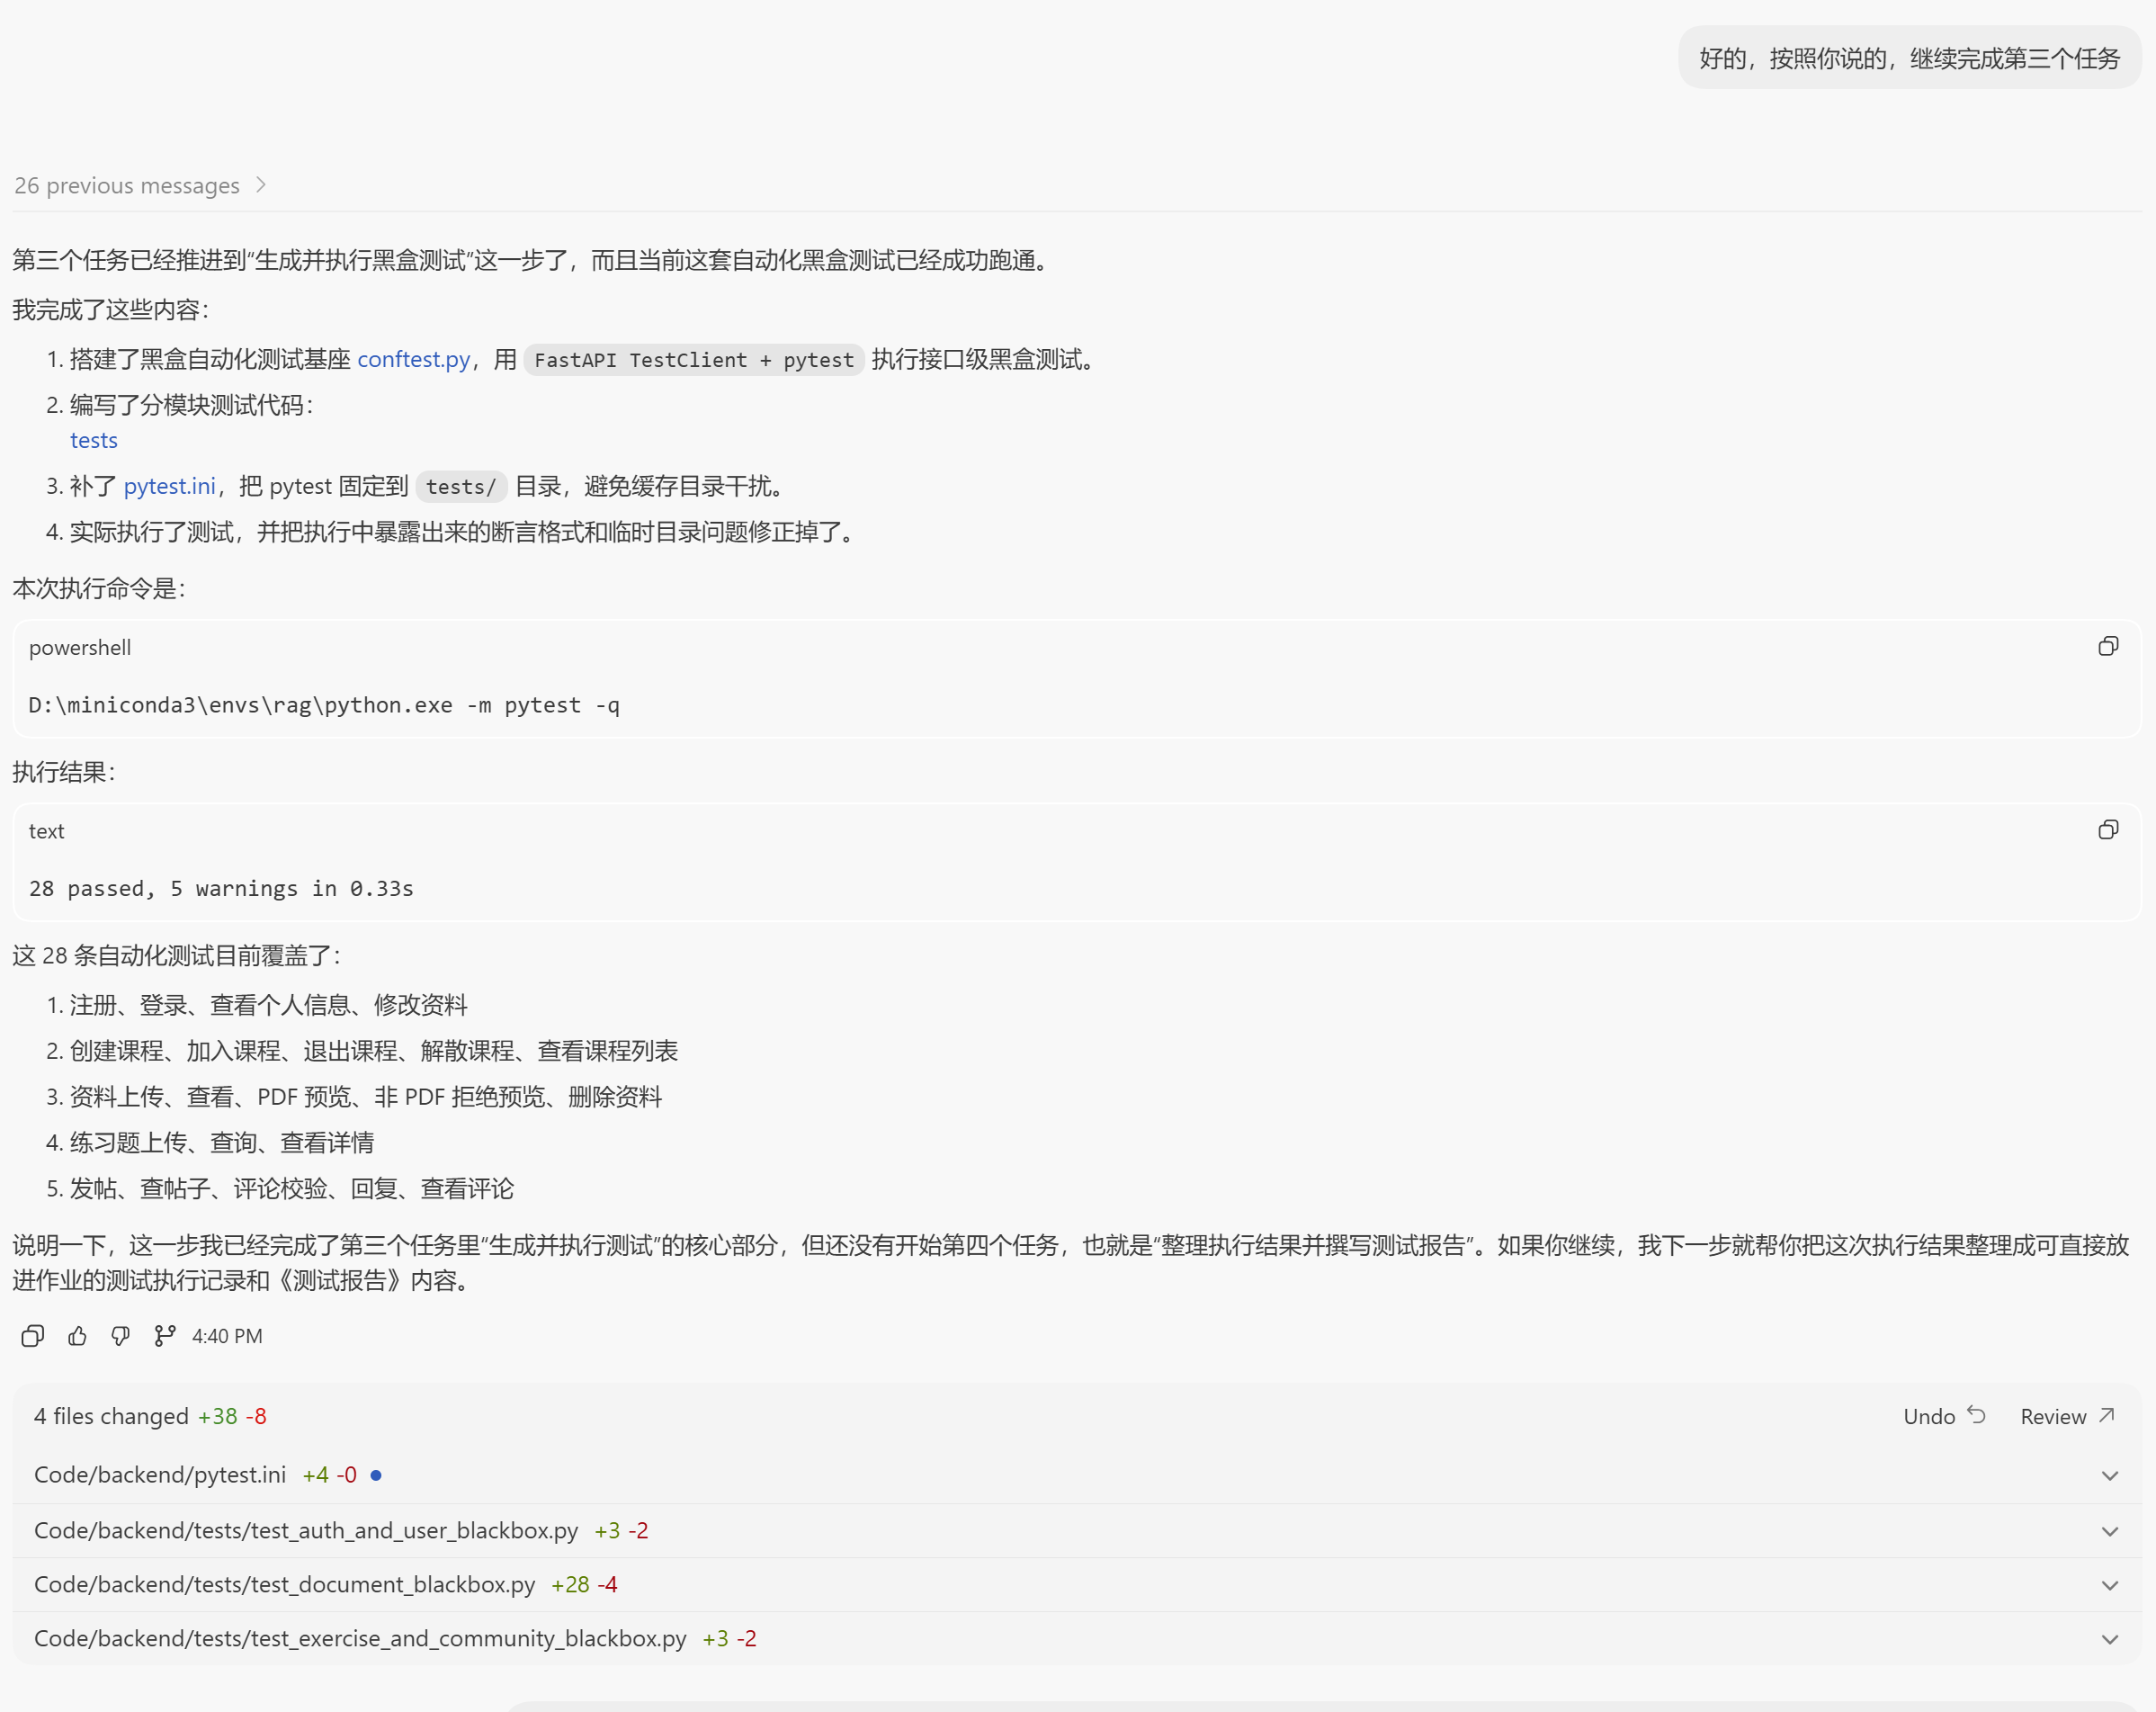
\includegraphics[width=0.92\textwidth]{任务3继续.png}
  \caption{任务三继续：继续第三项任务，模型搭建自动化黑盒测试代码并给出执行结果}
\end{figure}

\begin{figure}[H]
  \centering
  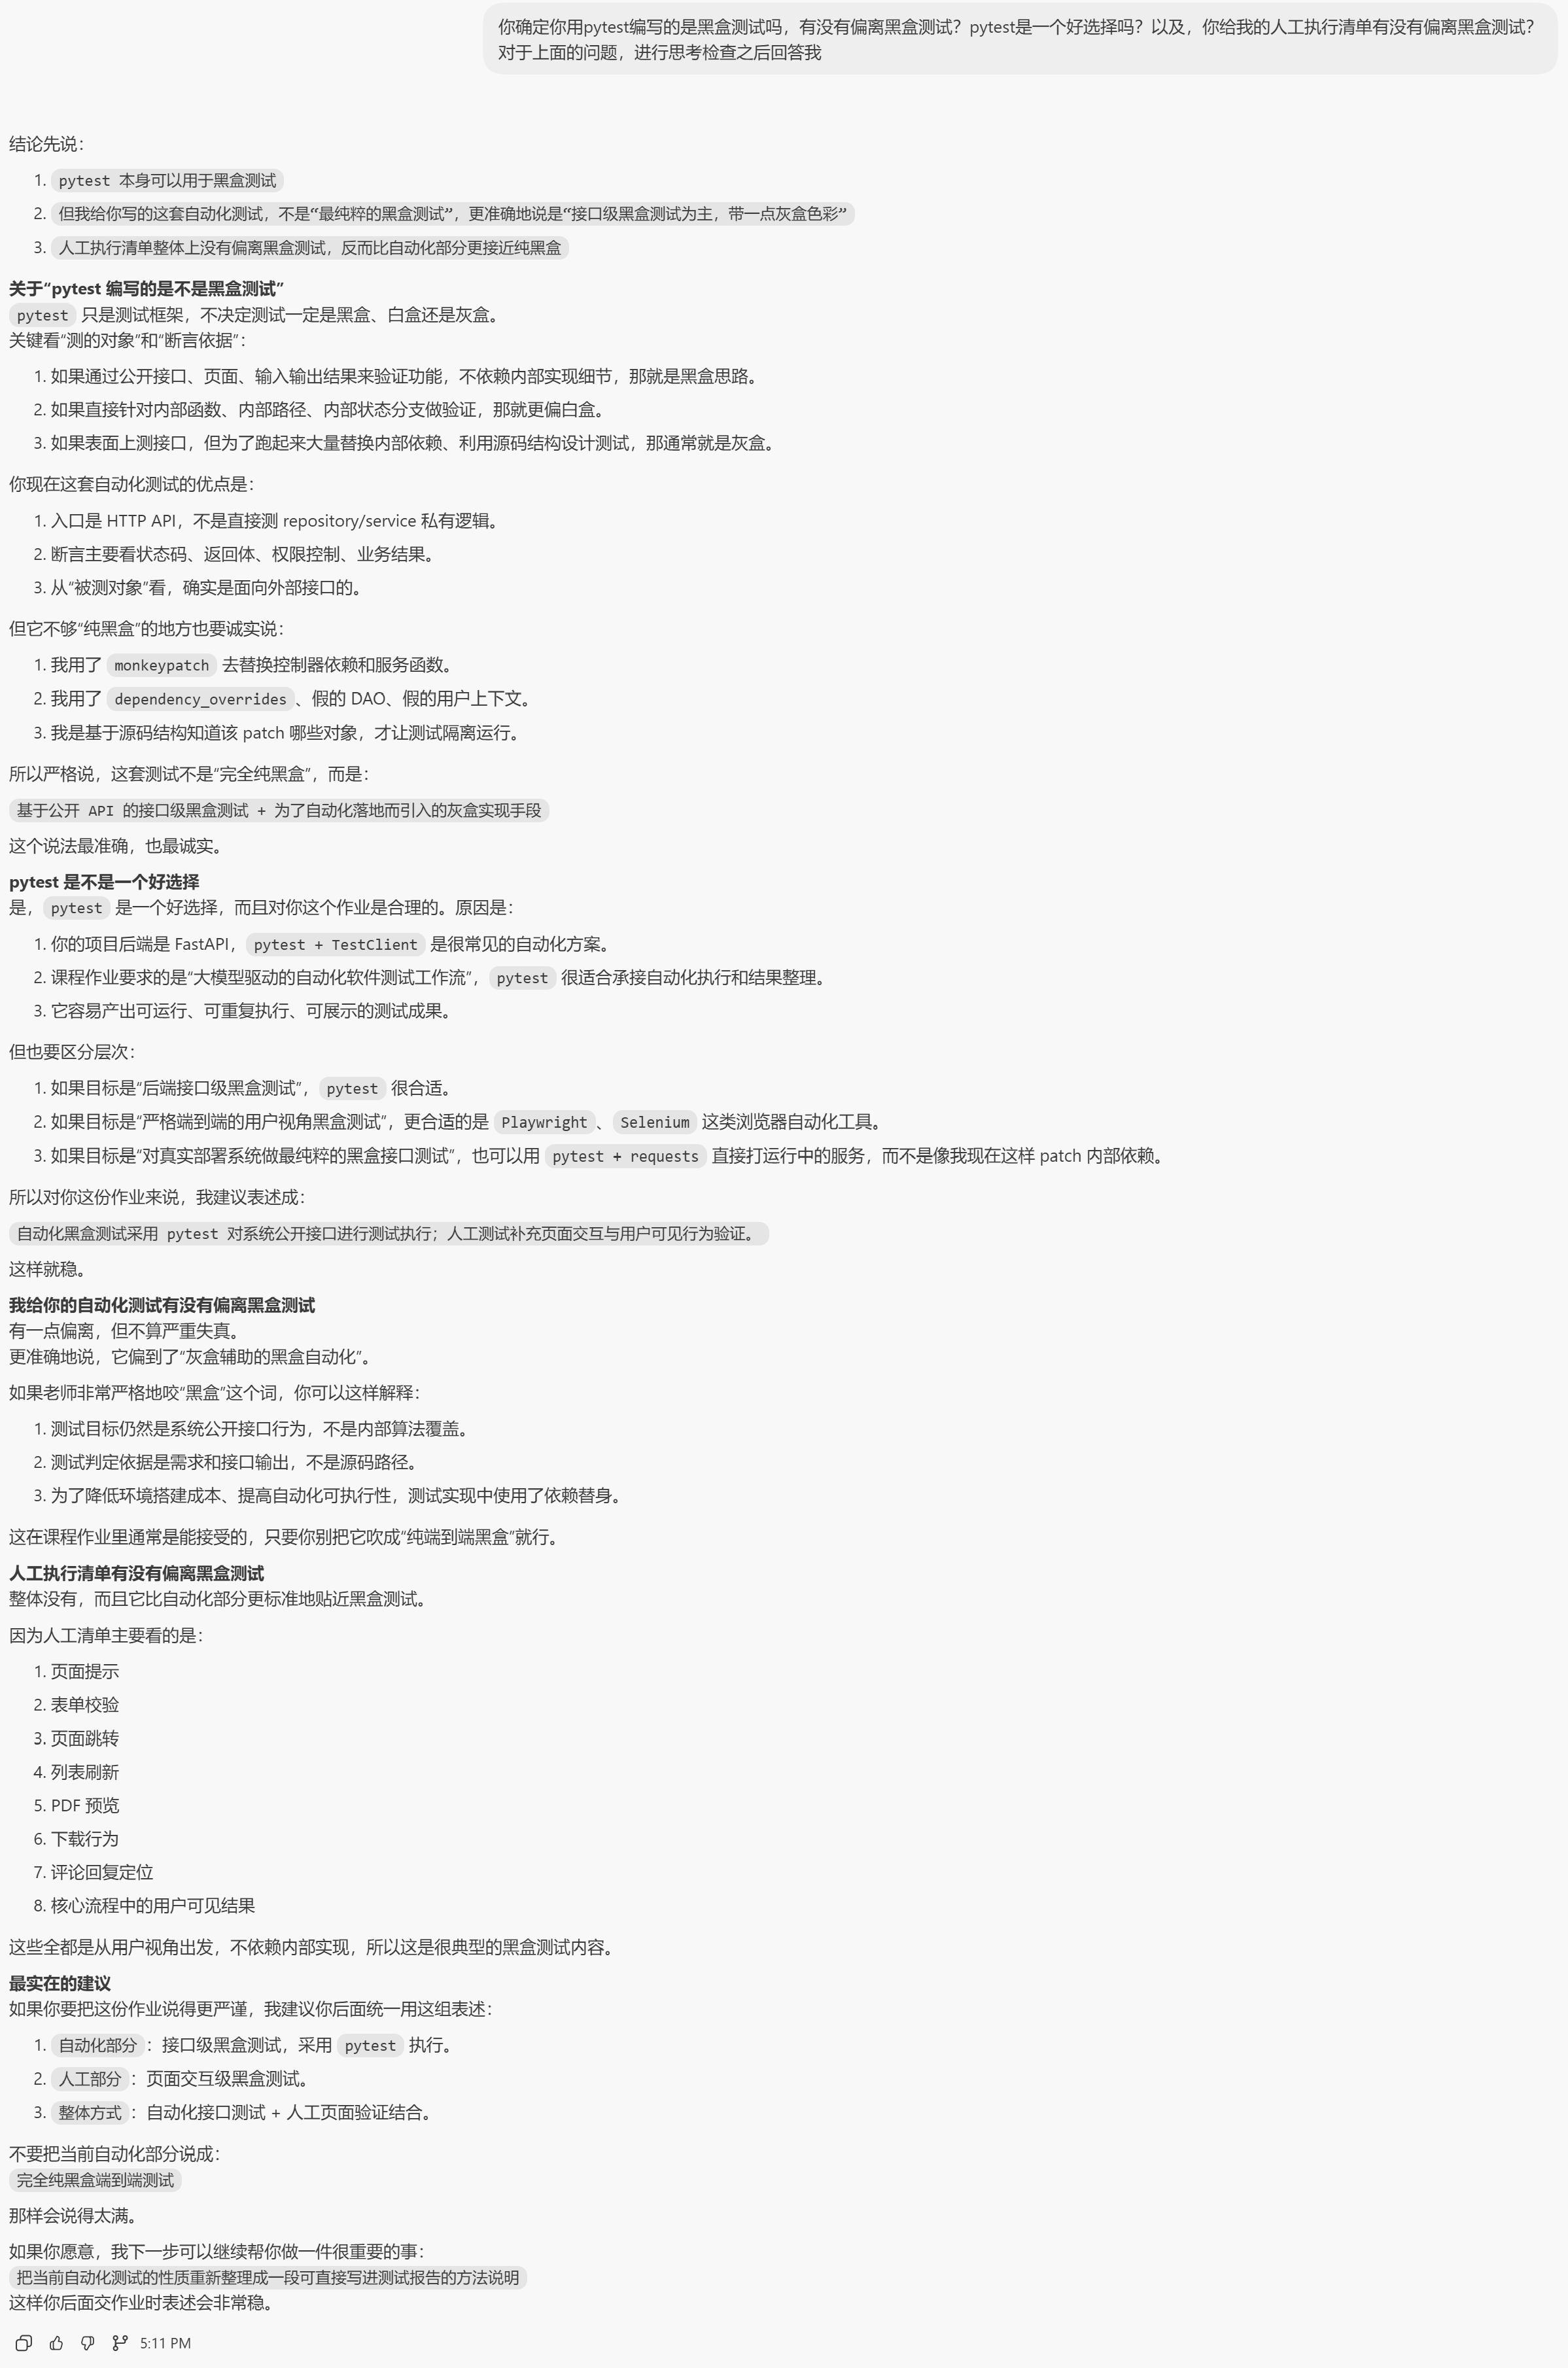
\includegraphics[width=0.92\textwidth]{任务3检验.png}
  \caption{任务三检验：继续检验 \texttt{pytest}、黑盒测试边界与人工测试定位}
\end{figure}

\begin{figure}[H]
  \centering
  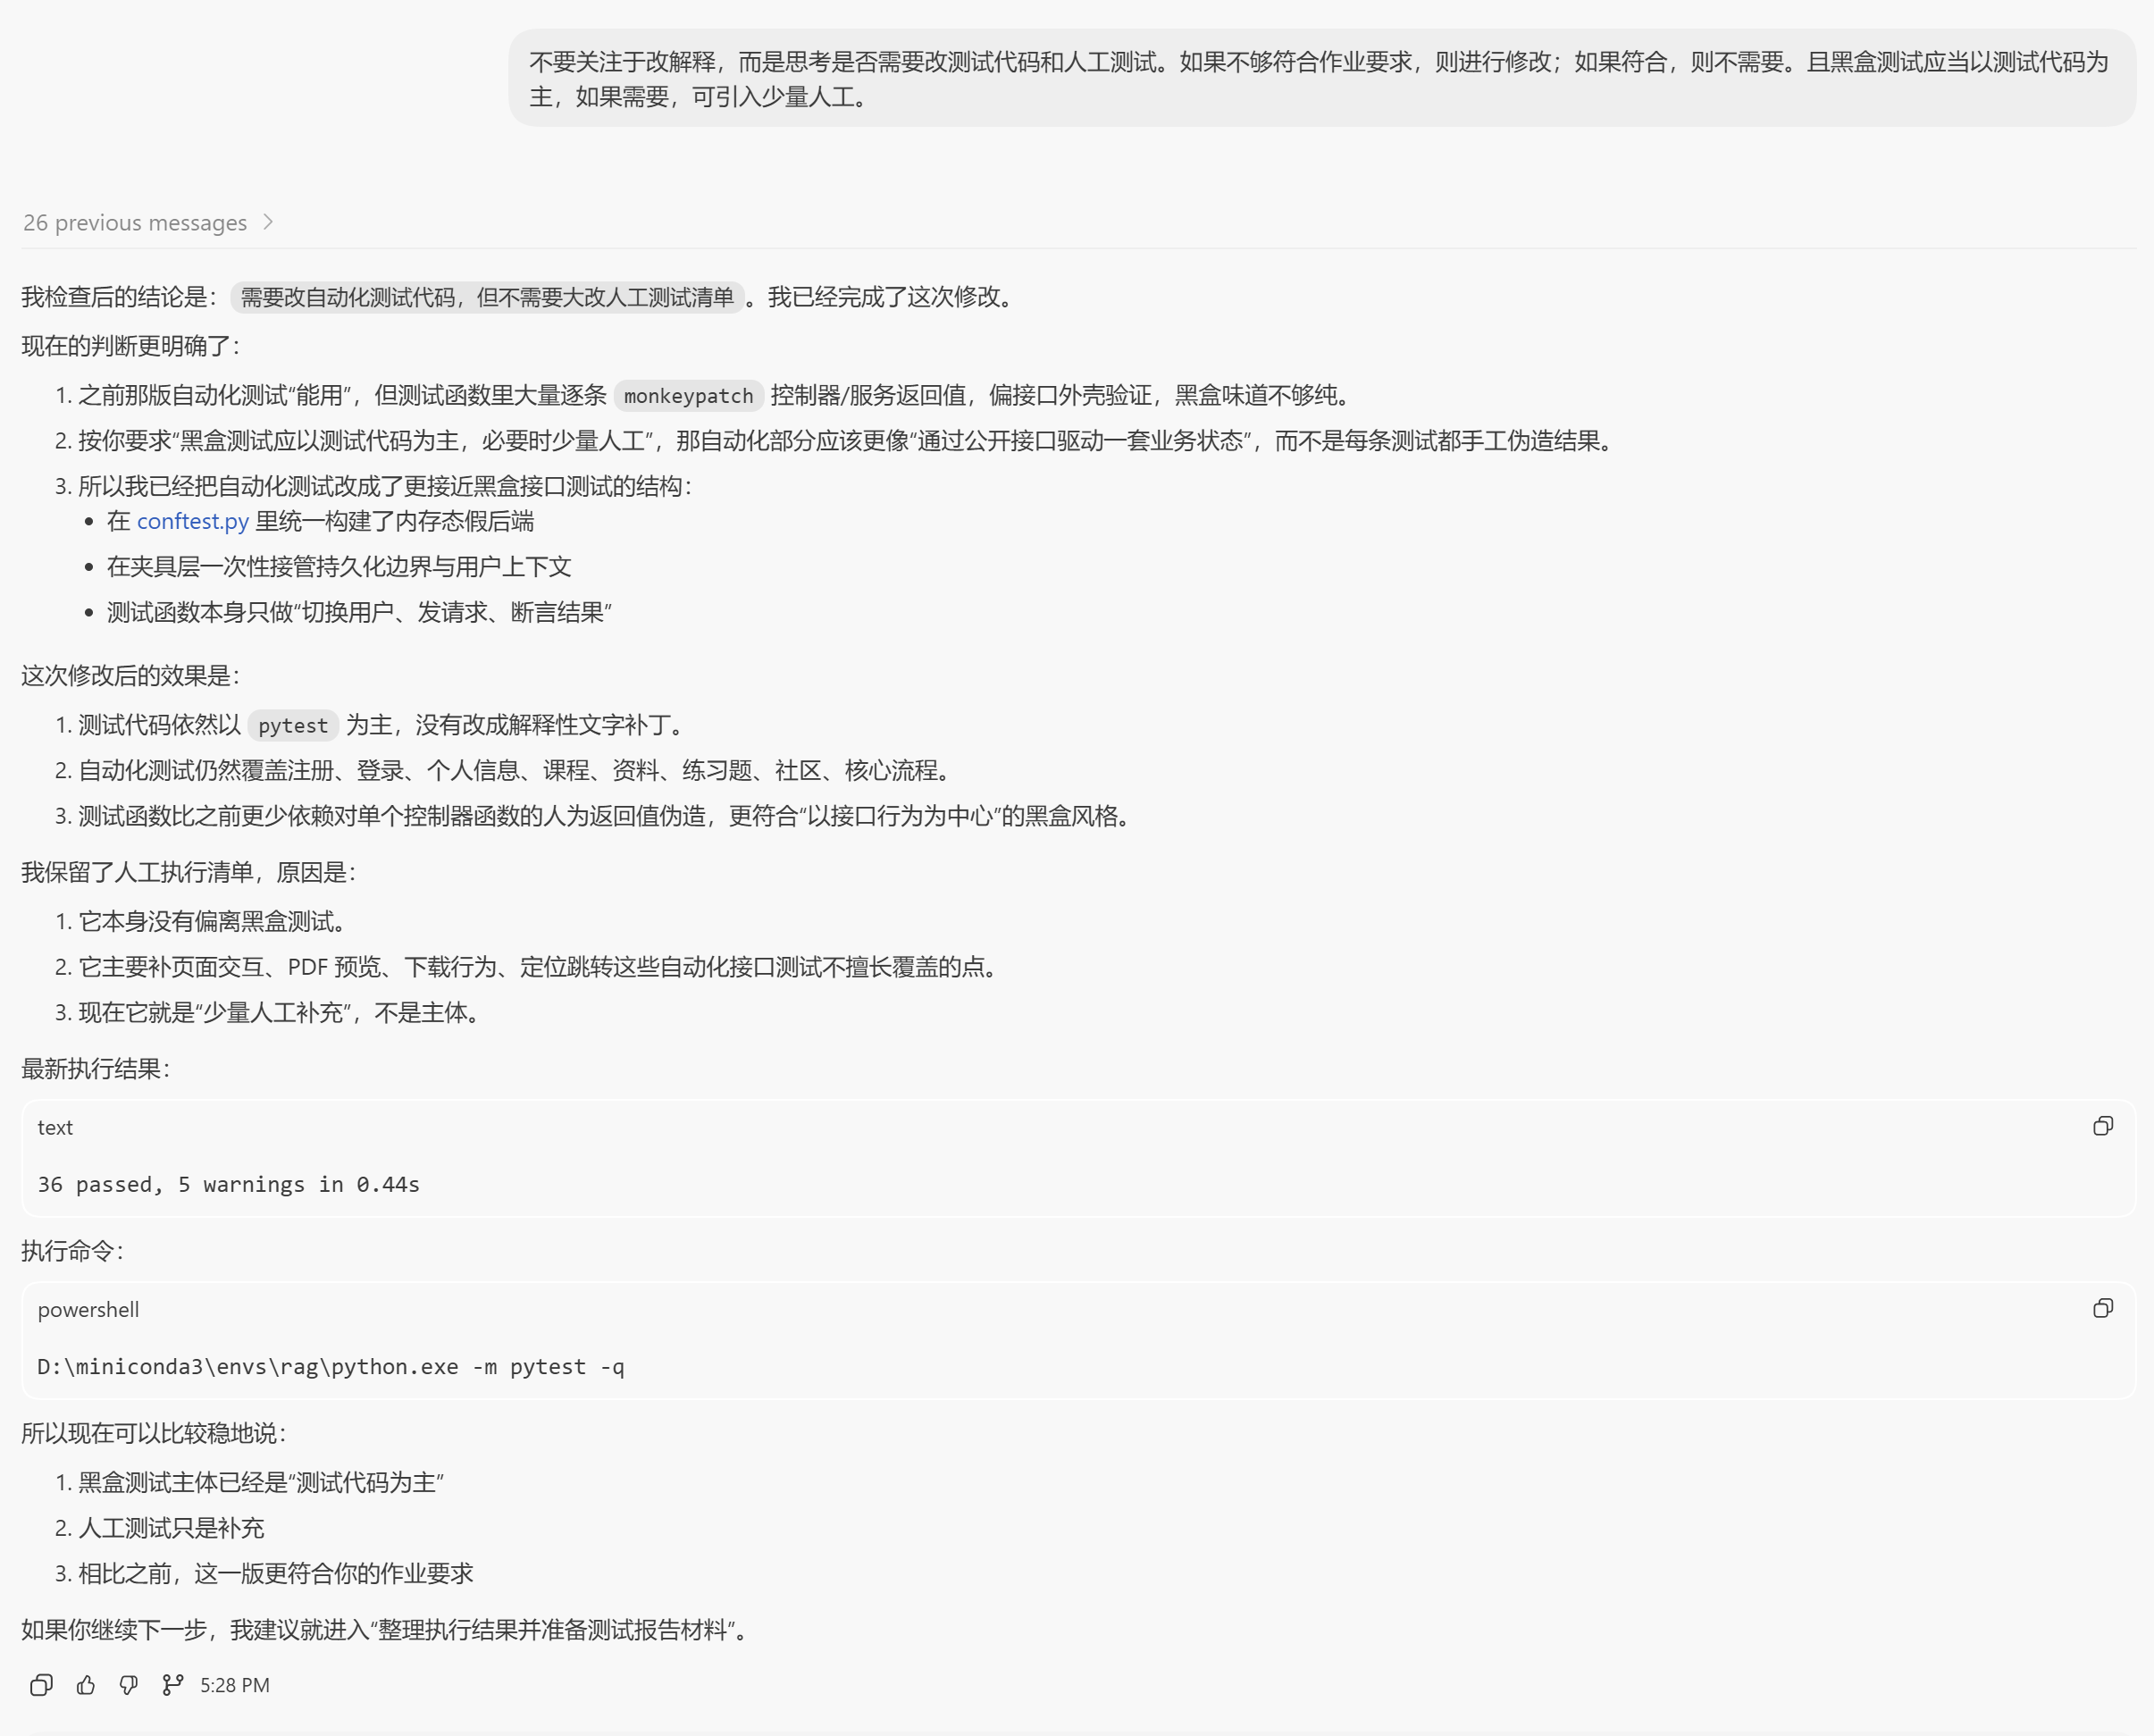
\includegraphics[width=0.92\textwidth]{任务3补充.png}
  \caption{任务三补充：补充说明课程作业要求与任务顺序之间的关系}
\end{figure}

\subsection{任务四：执行记录与测试报告}

这一阶段主要是整理测试执行记录、编写测试报告，并继续检查测试计划与测试报告是否存在冗余内容。模型根据执行结果汇总自动化测试与人工测试数据，并继续对文档结构和表述方式进行修改。

\begin{figure}[H]
  \centering
  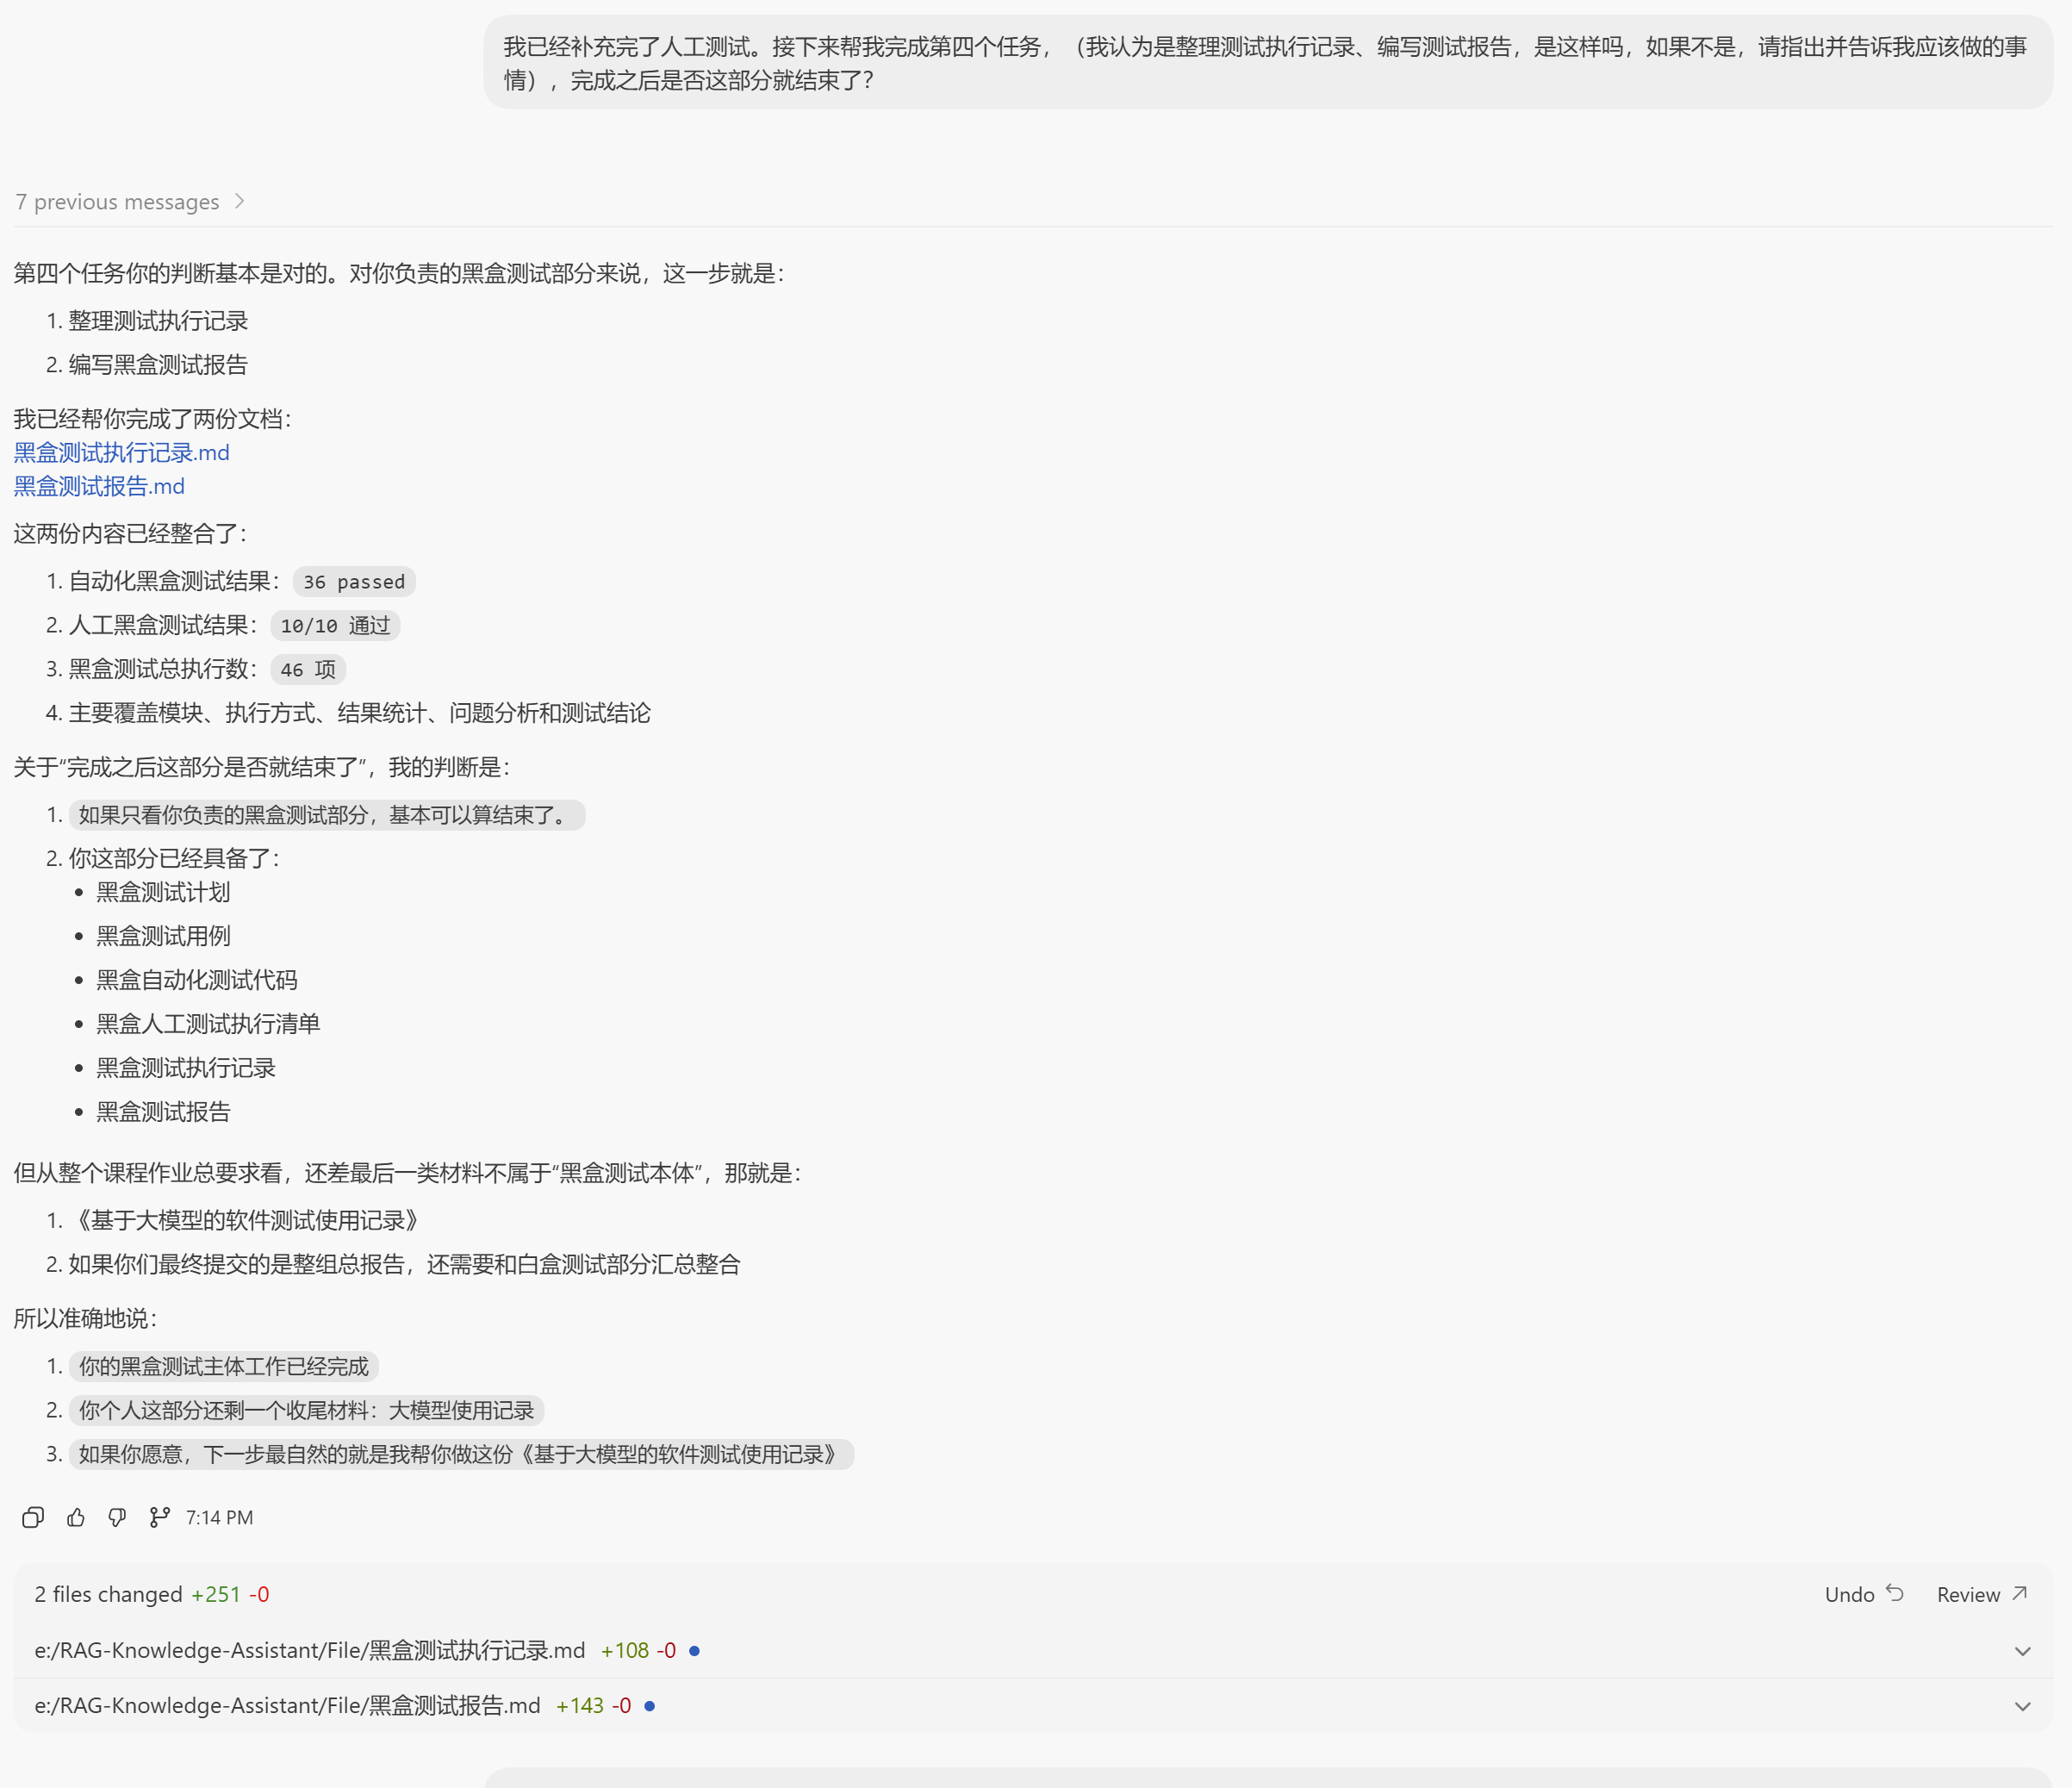
\includegraphics[width=0.92\textwidth]{任务4开始.png}
  \caption{任务四开始：整理测试执行记录并编写测试报告}
\end{figure}

\begin{figure}[H]
  \centering
  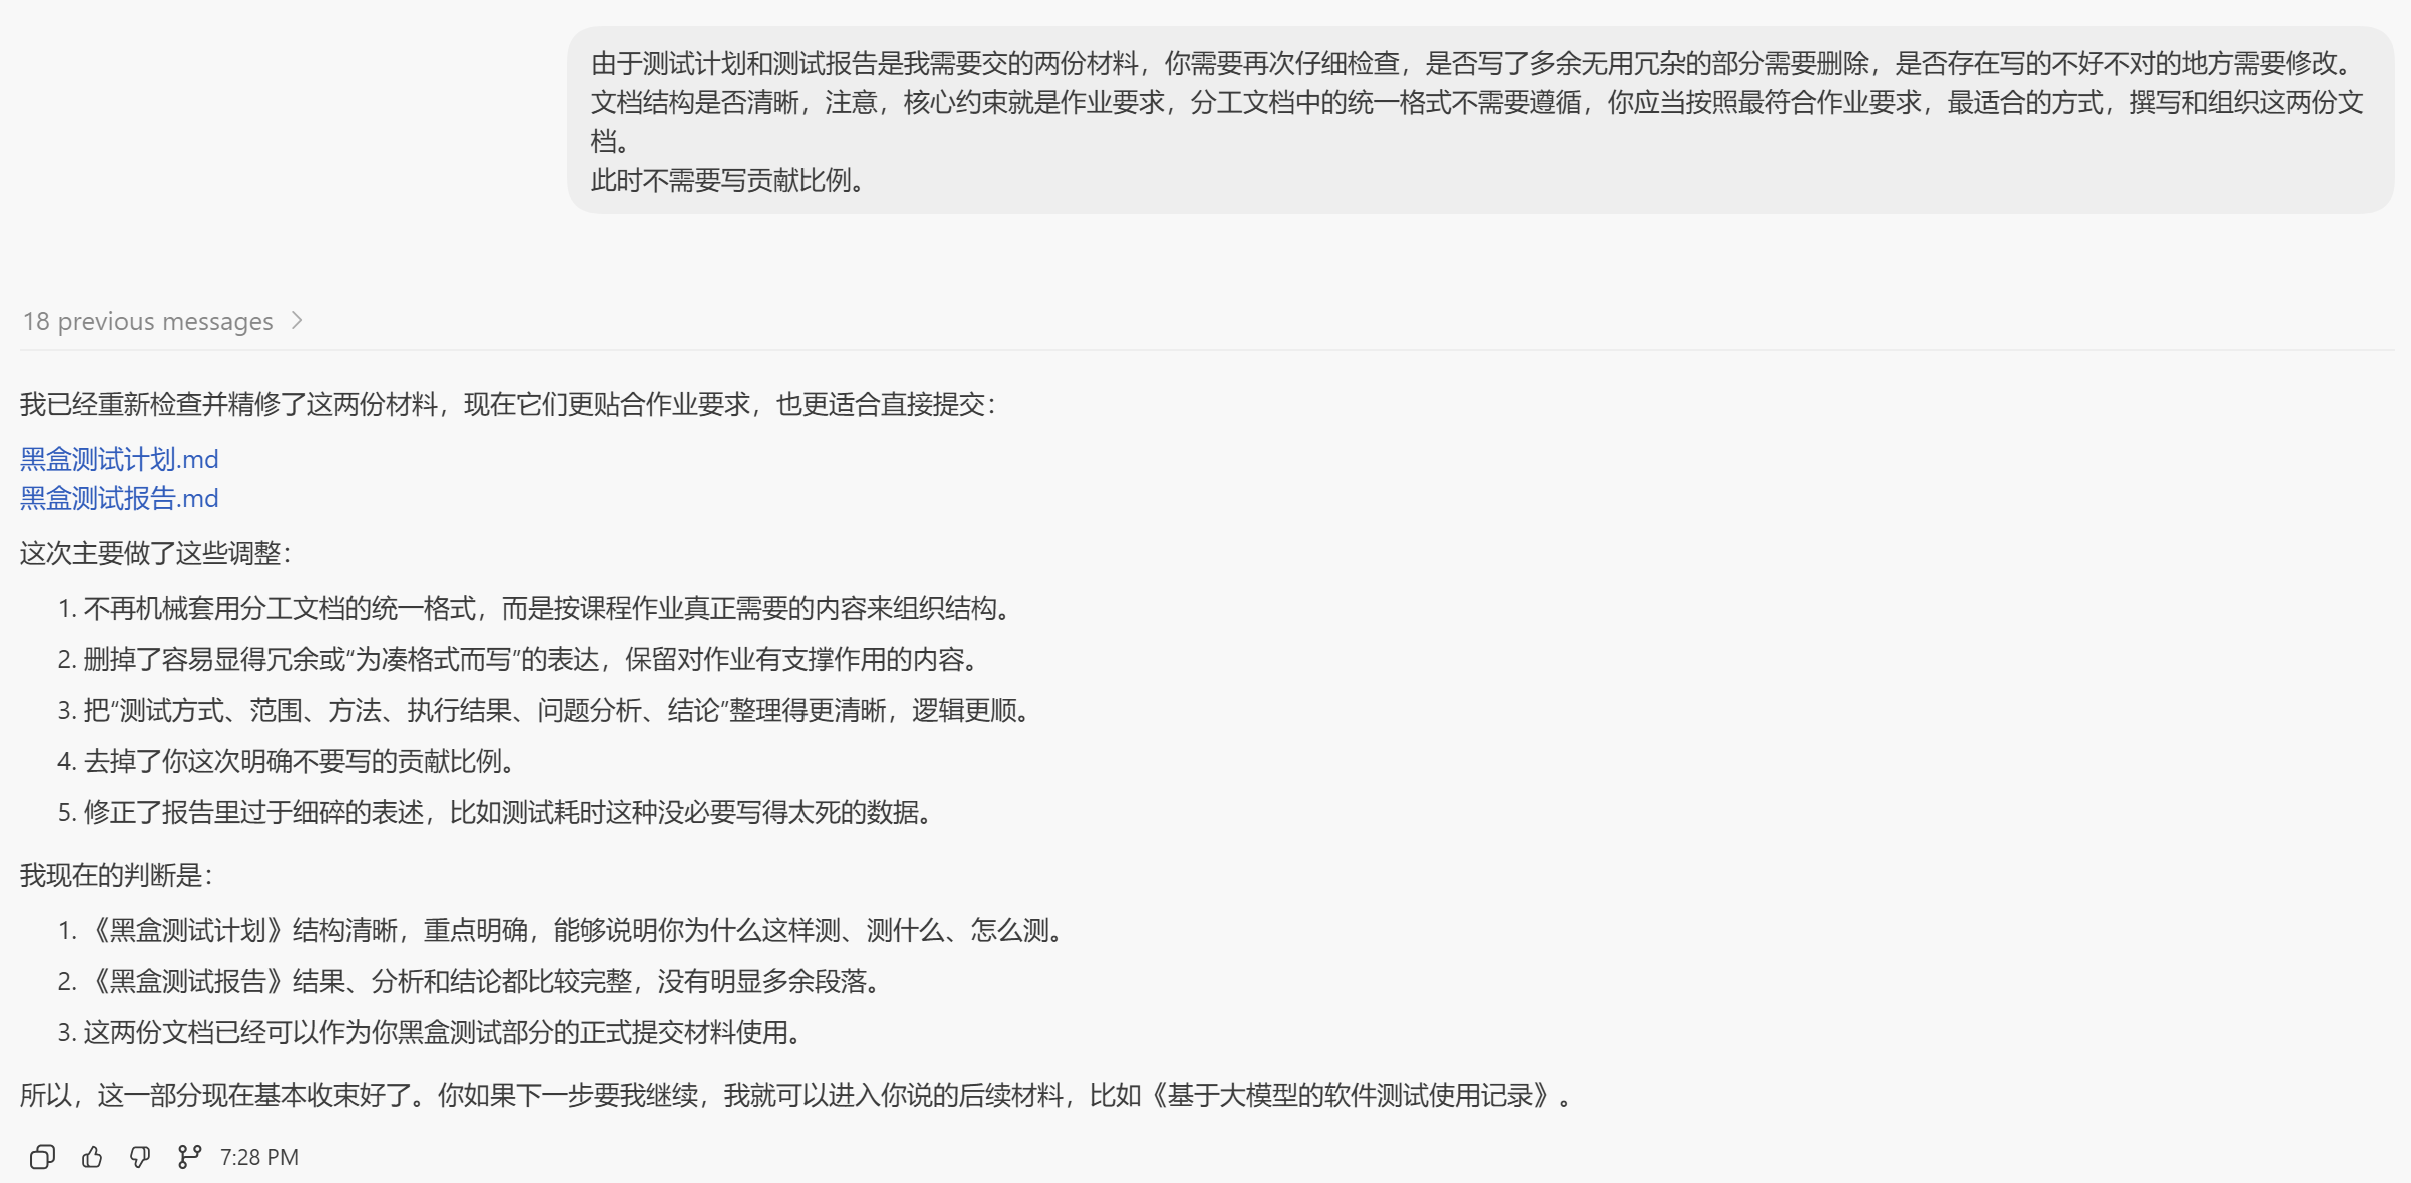
\includegraphics[width=0.92\textwidth]{任务4改进.png}
  \caption{任务四改进：继续检查并精修测试计划与测试报告}
\end{figure}


\section{白盒测试使用记录}

本节记录我与大模型协作完成白盒测试的关键交互过程，包含负责人一与负责人二两部分内容。由于历史对话较长，这里仅保留关键节点与代表性提示词。

\subsection{用户与认证、课程管理、课程资料管理}
\subsubsection{任务一：测试计划}

我先向模型提供课程作业要求、分工说明和现有文档状态，明确我作为白盒负责人一的身份。模型据此先读取《小组分工与文档格式》《测试计划》与《需求说明文档》及相关代码，然后确认白盒计划应围绕我负责的后端核心链路展开。

\begin{figure}[htbp]
  \centering
  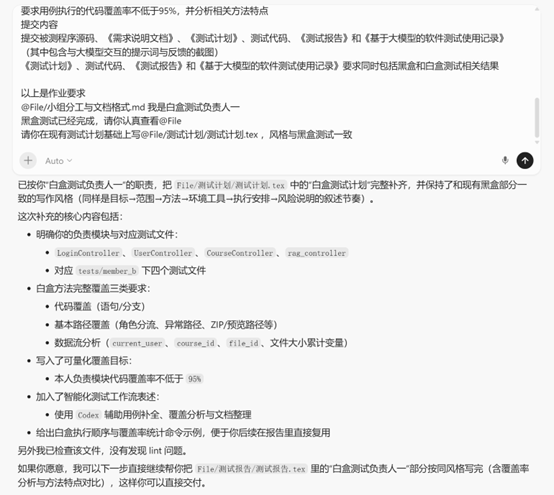
\includegraphics[width=0.8\textwidth]{白盒测试对话截图1/测试计划生成.png}
  \caption{测试计划初步生成：提供作业要求、成员分工与当前文档状态}
  \label{fig:test-plan-generation}
\end{figure}

我发现模型对白盒测试的理解有一定偏离，我要求它不要对每层进行单独测试，而是贯通controller->service->dao->repository层。

\begin{figure}[H]
  \centering
  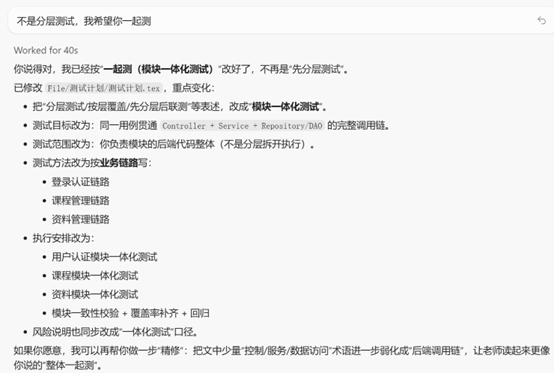
\includegraphics[width=0.8\textwidth]{白盒测试对话截图1/测试计划迭代1.png}
  \caption{测试计划迭代：明确贯通测试的需求}
\end{figure}

我要求模型将覆盖率、基本路径、数据流三类方法都要落地。

\begin{figure}[H]
  \centering
  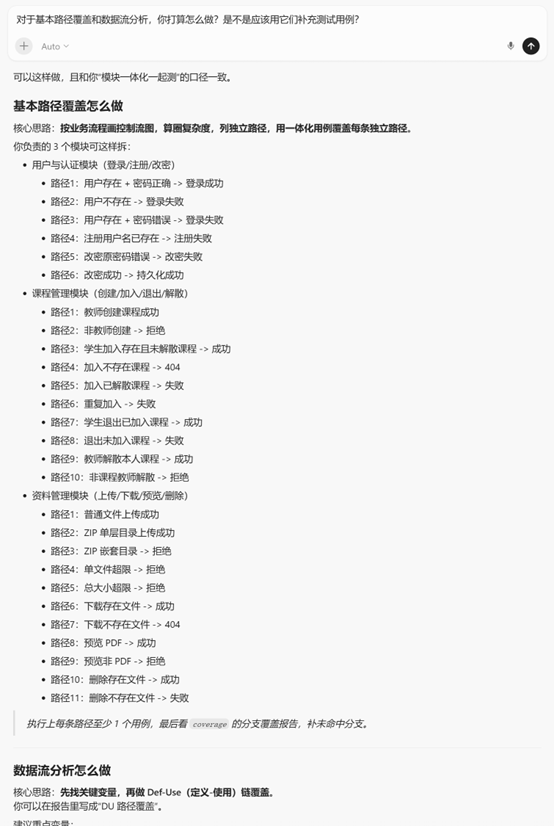
\includegraphics[width=0.8\textwidth]{白盒测试对话截图1/测试计划迭代2.png}
  \caption{测试计划迭代：根据基本路径及数据流完善测试}
\end{figure}

我还进行了一些追问，模型持续修正细节，我也在问答中深化了我对白盒测试核心逻辑的理解（图略）。

\subsubsection{任务二：测试代码生成、执行、失败定位与修复}

进入执行阶段后，模型按我负责范围运行 \texttt{pytest} 并回看失败栈，完成修复，最后重新执行回归确认。

\begin{figure}[H]
  \centering
  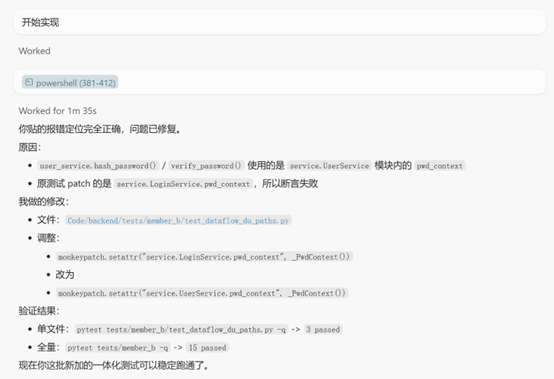
\includegraphics[width=0.8\textwidth]{白盒测试对话截图1/测试代码生成.png}
  \caption{测试代码生成及修复}
\end{figure}

由于测试代码对dao, repository层的覆盖率不足，模型试图对它们进行单独测试，被我阻止，澄清贯通测试的需求。

\begin{figure}[H]
  \centering
  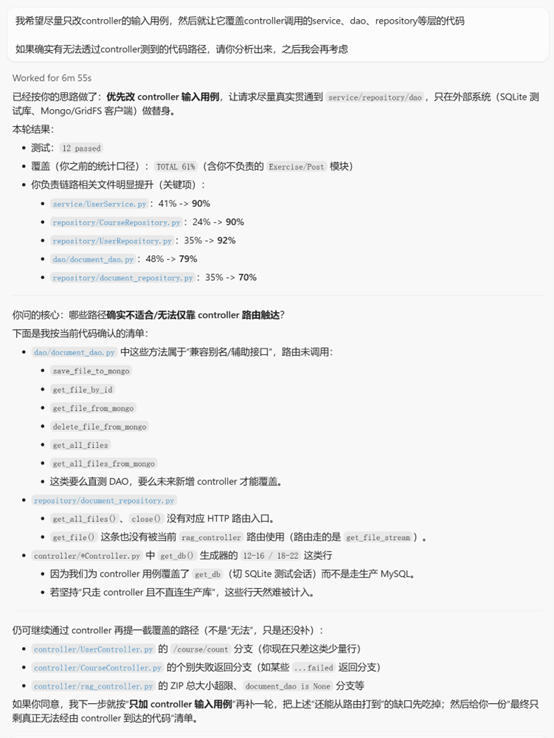
\includegraphics[width=0.8\textwidth]{白盒测试对话截图1/测试覆盖率提高.png}
  \caption{澄清测试覆盖率提高方法}
\end{figure}

让模型补完用例后自己运行并查看覆盖率，如果没有命中的部分还能靠补用例来命中，就继续补充，直到未命中部分都是真正无法到达的代码。同时，分析未覆盖原因。

{\centering
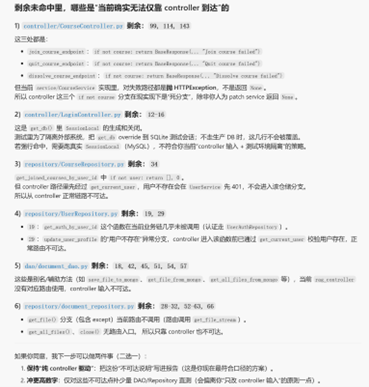
\includegraphics[width=0.8\textwidth]{白盒测试对话截图1/未命中原因.png}
\captionof{figure}{未覆盖原因}
\par}

\subsubsection{任务三：执行记录与测试报告}

在覆盖率达到要求后，我要求模型根据测试结果，生成测试报告。

\begin{figure}[H]
  \centering
  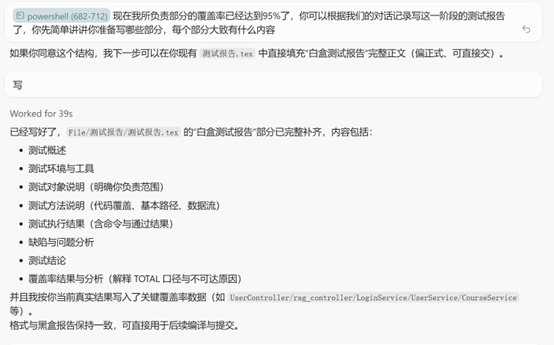
\includegraphics[width=0.8\textwidth]{白盒测试对话截图1/测试报告.png}
  \caption{测试报告}
\end{figure}

调整测试报告。

\begin{figure}[H]
  \centering
  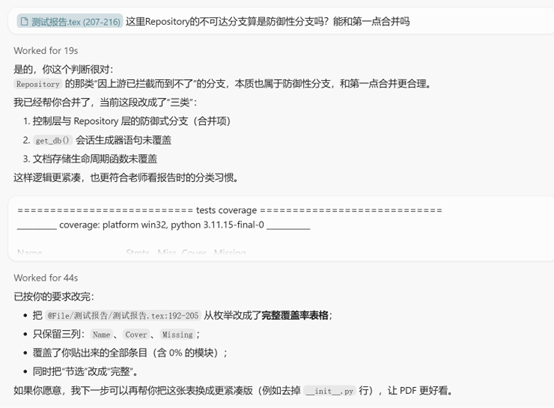
\includegraphics[width=0.8\textwidth]{白盒测试对话截图1/测试报告修改.png}
  \caption{测试报告修改}
\end{figure}

\subsection{练习管理与课程社区模块}

\subsubsection{任务一：测试计划}

我先提供了作业要求、个人分工与任务顺序，要求模型严格按顺序执行；随后对《测试计划-白盒测试-练习与社区模块》进行精修，删除冗余描述并保留必要边界说明。

\begin{figure}[H]
  \centering
  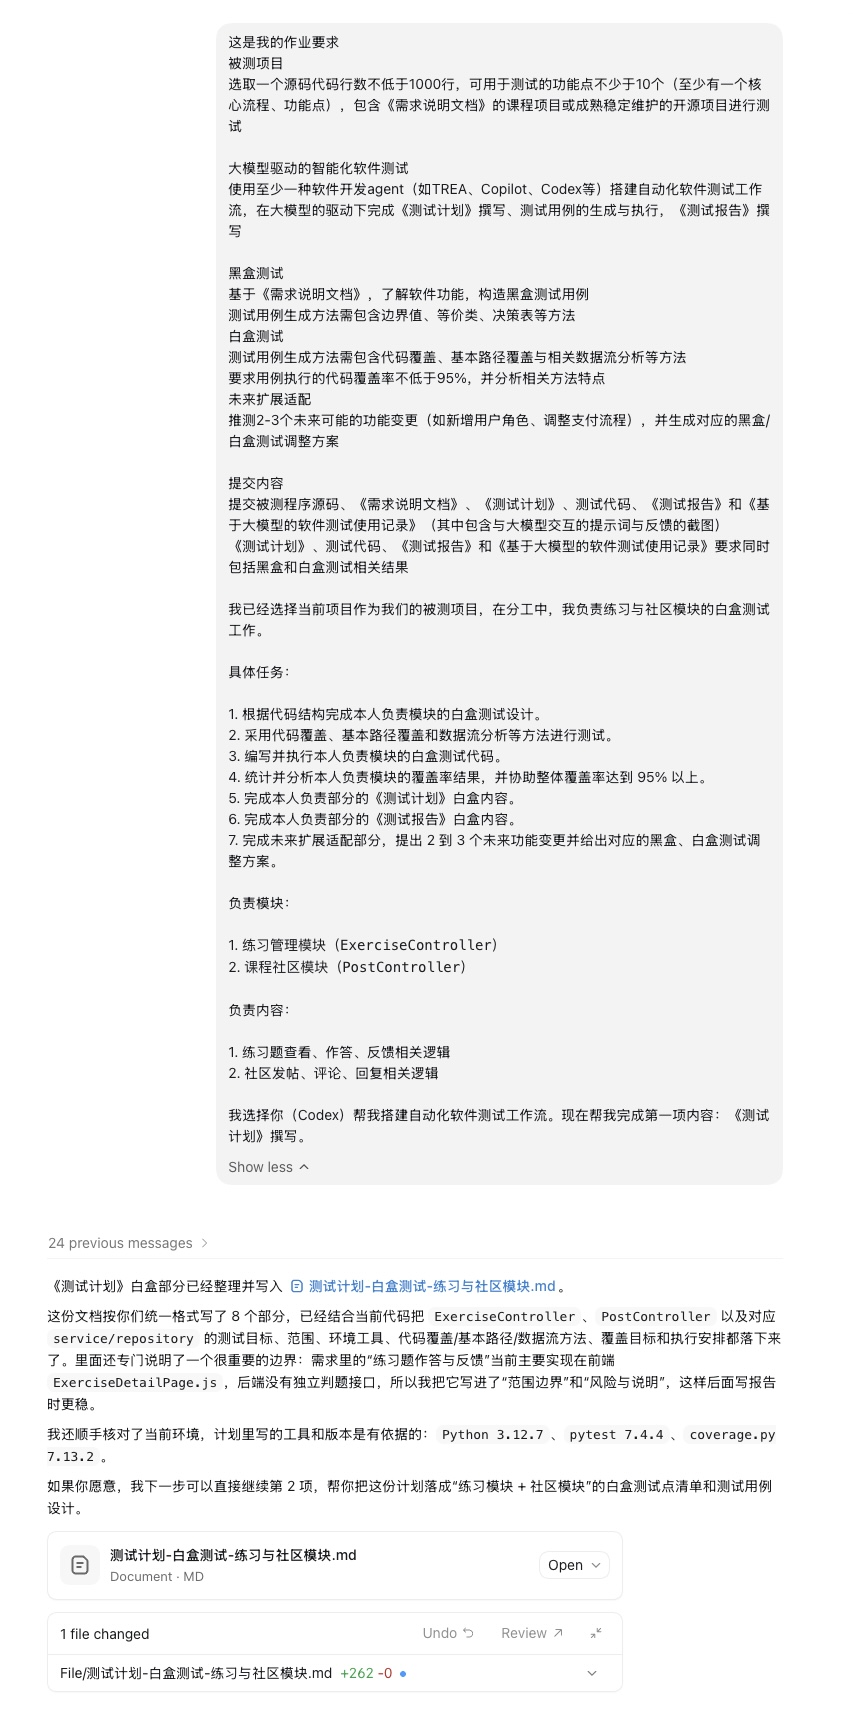
\includegraphics[width=0.7\textwidth]{白盒测试2对话截图/任务1-测试计划-1.png}
  \caption{任务一：提供作业要求与分工，启动测试计划}
\end{figure}

\begin{figure}[H]
  \centering
  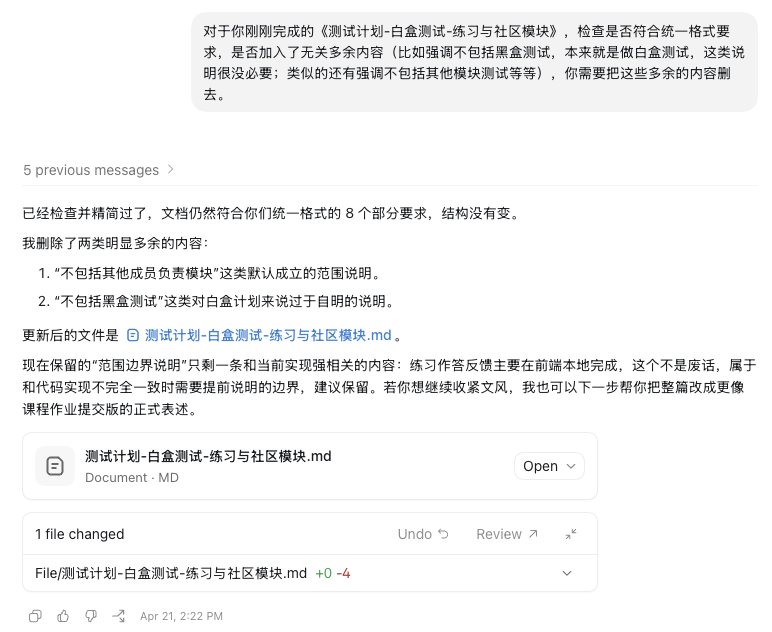
\includegraphics[width=0.82\textwidth]{白盒测试2对话截图/任务1-测试计划-2-修改.png}
  \caption{任务一：按统一格式精修测试计划并删除冗余内容}
\end{figure}

\subsubsection{任务二：构造测试用例}

在仅推进第二项任务的约束下，模型完成两个模块白盒用例集：练习模块 12 个、社区模块 11 个，另含 3 个缺陷触发补充用例，并对每个用例给出输入、步骤与预期结果。

\begin{figure}[H]
  \centering
  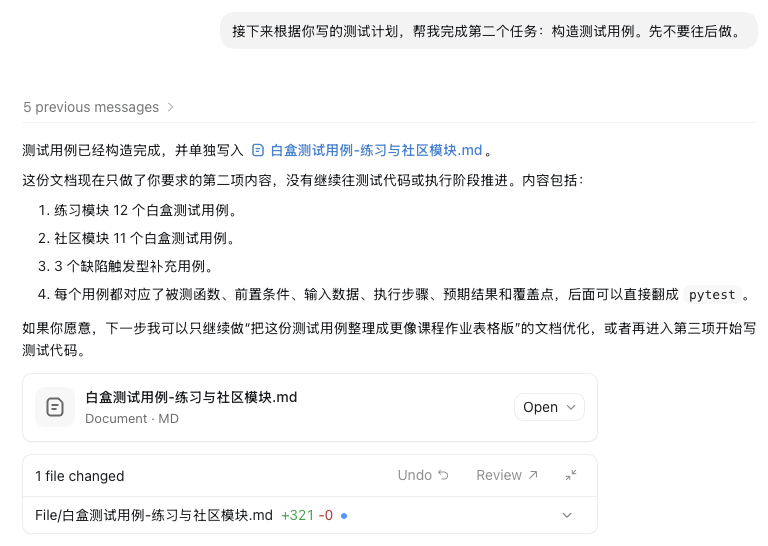
\includegraphics[width=0.82\textwidth]{白盒测试2对话截图/任务2-构造测试用例-1.png}
  \caption{任务二：构造练习与社区模块白盒测试用例}
\end{figure}

\subsubsection{任务三：编写并执行测试代码}

根据已构造用例，模型在 \texttt{conftest.py}、\texttt{test\_exercise\_module.py}、\texttt{test\_post\_module.py} 等文件落地测试并执行。初始结果为 \texttt{23 passed, 3 xfailed}。随后我发现了\texttt{xfailed}和之前知道的 \texttt{failed}不一样，于是追问了 \texttt{xfailed} 与 \texttt{failed} 的语义差异，并要求把缺陷用例改为普通失败以便在报告中直观展示真实缺陷。

\begin{figure}[H]
  \centering
  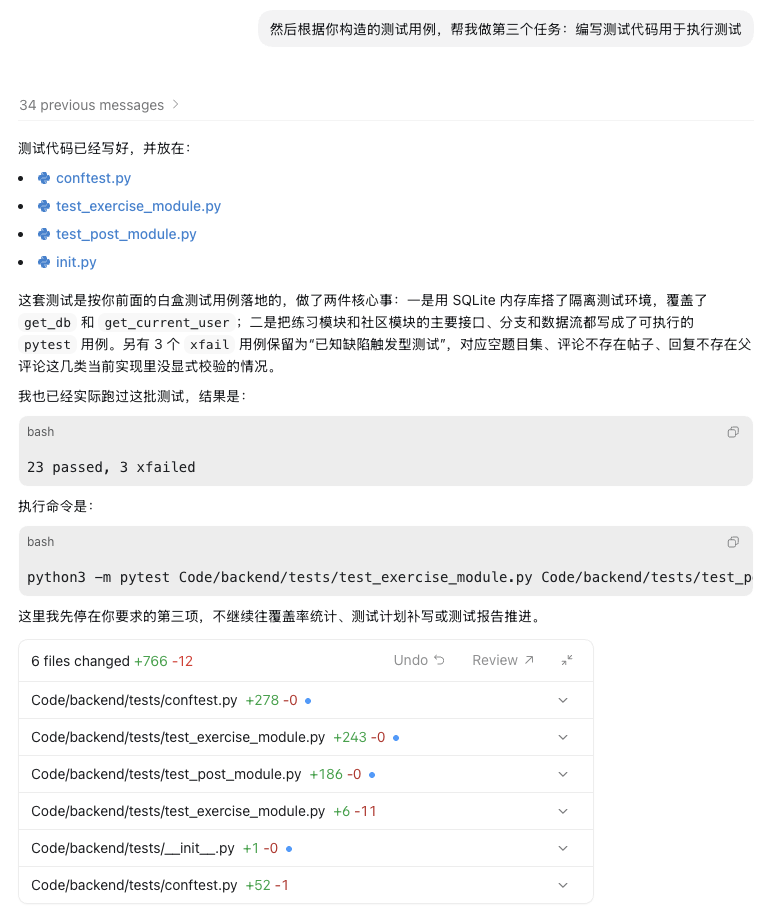
\includegraphics[width=0.82\textwidth]{白盒测试2对话截图/任务3-编写测试代码-1.png}
  \caption{任务三：测试代码生成与首轮执行（23 passed, 3 xfailed）}
\end{figure}

\begin{figure}[H]
  \centering
  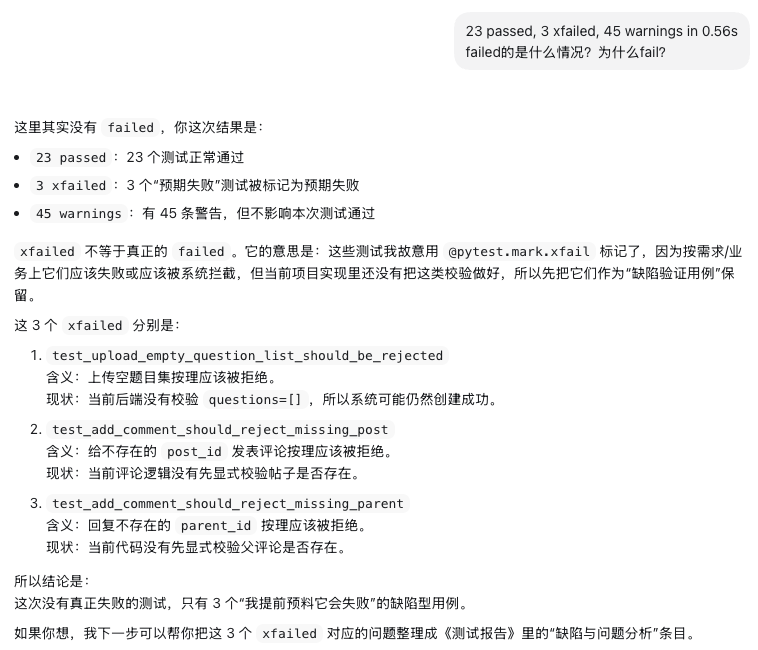
\includegraphics[width=0.82\textwidth]{白盒测试2对话截图/任务3-编写测试代码-2-fail情况.png}
  \caption{任务三：追问 xfailed 的含义与缺陷对应关系}
\end{figure}

\begin{figure}[H]
  \centering
  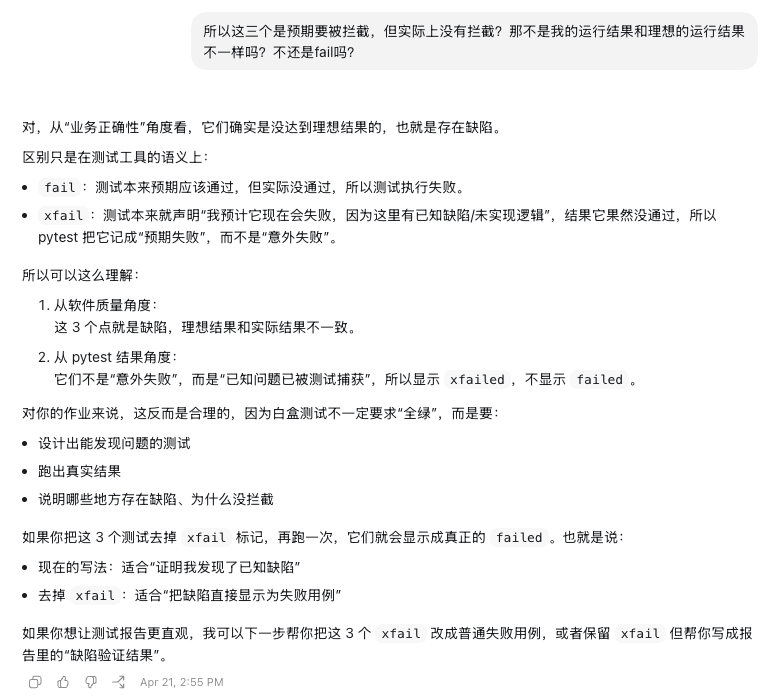
\includegraphics[width=0.82\textwidth]{白盒测试2对话截图/任务3-编写测试代码-3-fail追问.png}
  \caption{任务三：澄清 xfailed 与 failed 的质量语义差异}
\end{figure}

\begin{figure}[H]
  \centering
  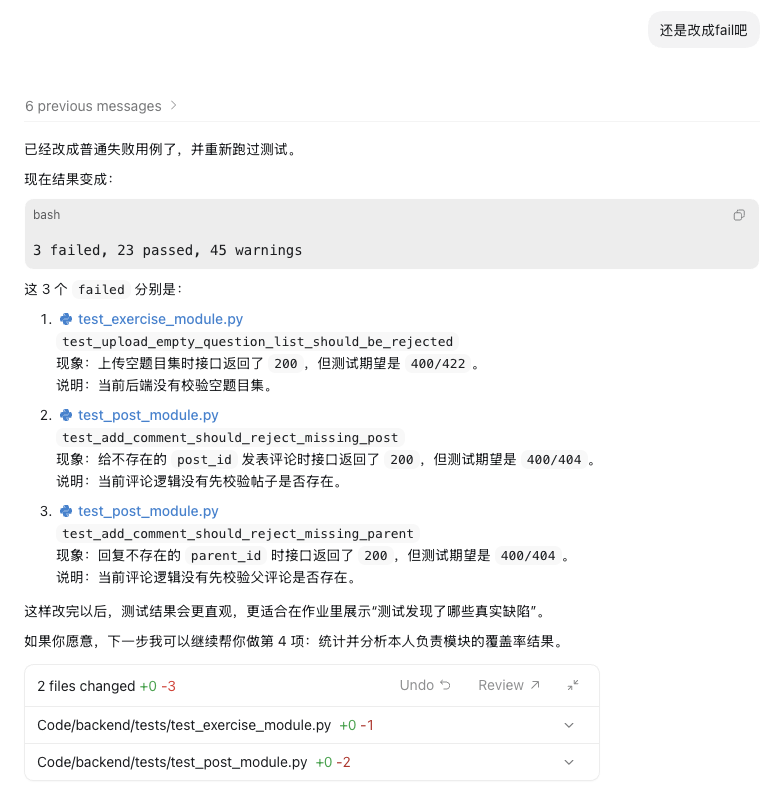
\includegraphics[width=0.82\textwidth]{白盒测试2对话截图/任务3-编写测试代码-4-fail修改.png}
  \caption{任务三：将 xfailed 改为 failed，结果变为 3 failed, 23 passed}
\end{figure}

\subsubsection{任务四：覆盖率统计与分析}

我要求模型先判断下一步任务，模型确认应先做覆盖率统计与分析，再进入报告撰写。随后执行 \texttt{coverage} 并分析：我负责范围内覆盖率达到 100\%。

\begin{figure}[H]
  \centering
  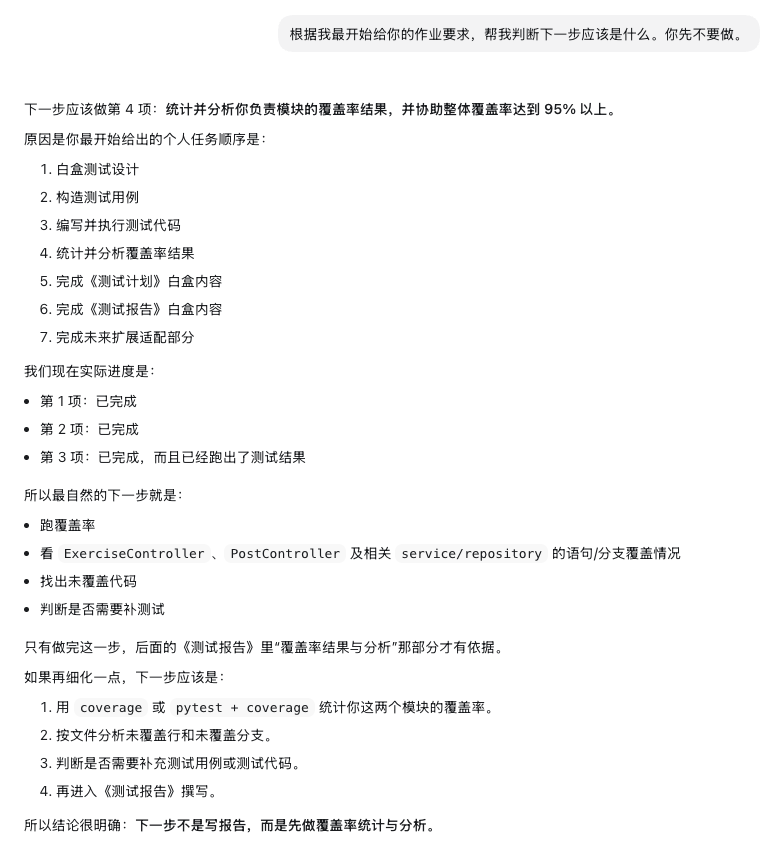
\includegraphics[width=0.82\textwidth]{白盒测试2对话截图/任务4-覆盖率-1.png}
  \caption{任务四：确认先做覆盖率统计与分析}
\end{figure}

\begin{figure}[H]
  \centering
  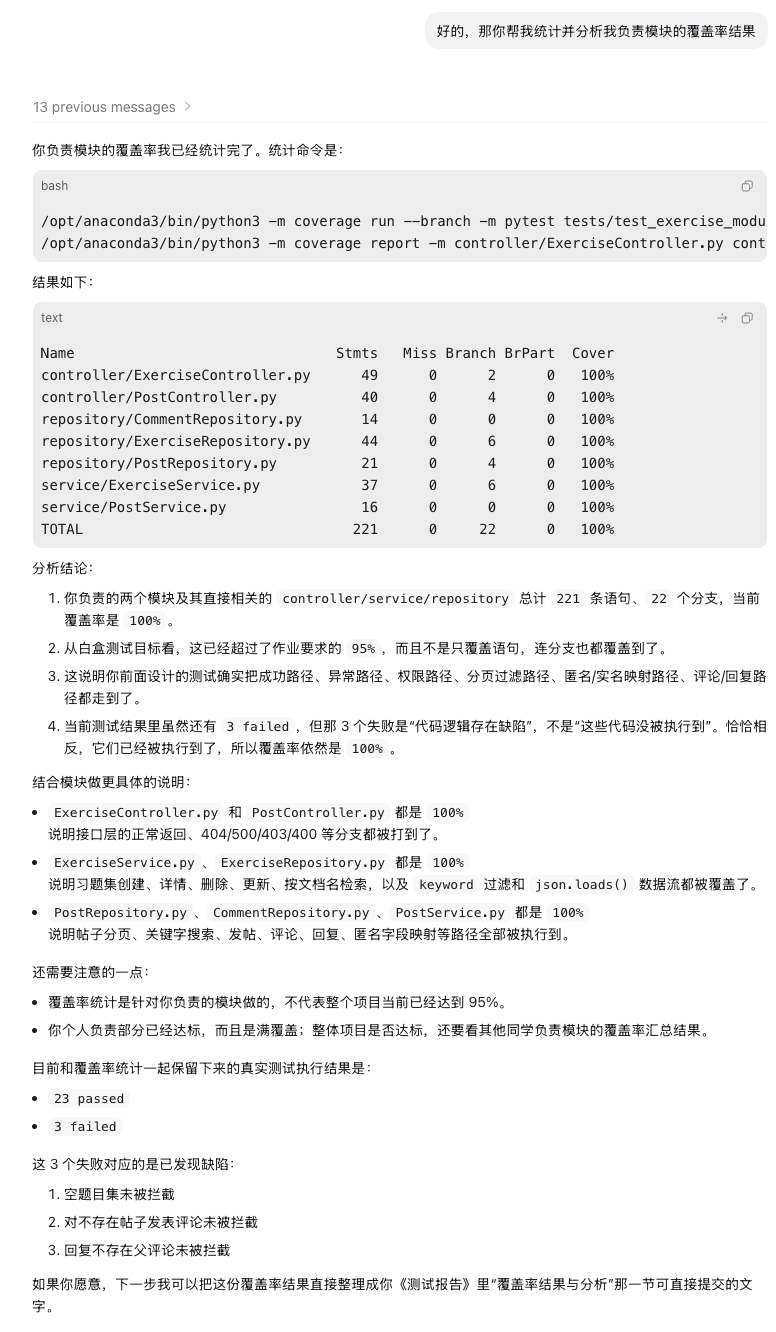
\includegraphics[width=0.82\textwidth]{白盒测试2对话截图/任务4-覆盖率-2-测试.png}
  \caption{任务四：覆盖率统计结果与分析}
\end{figure}

\subsubsection{任务五：测试报告与结果合并}

覆盖率分析完成后，我要求模型按统一模板撰写《测试报告-白盒测试-练习与社区模块》，并进一步把新增内容合并回测试计划与测试报告，保证结构一致、口径一致。

\begin{figure}[H]
  \centering
  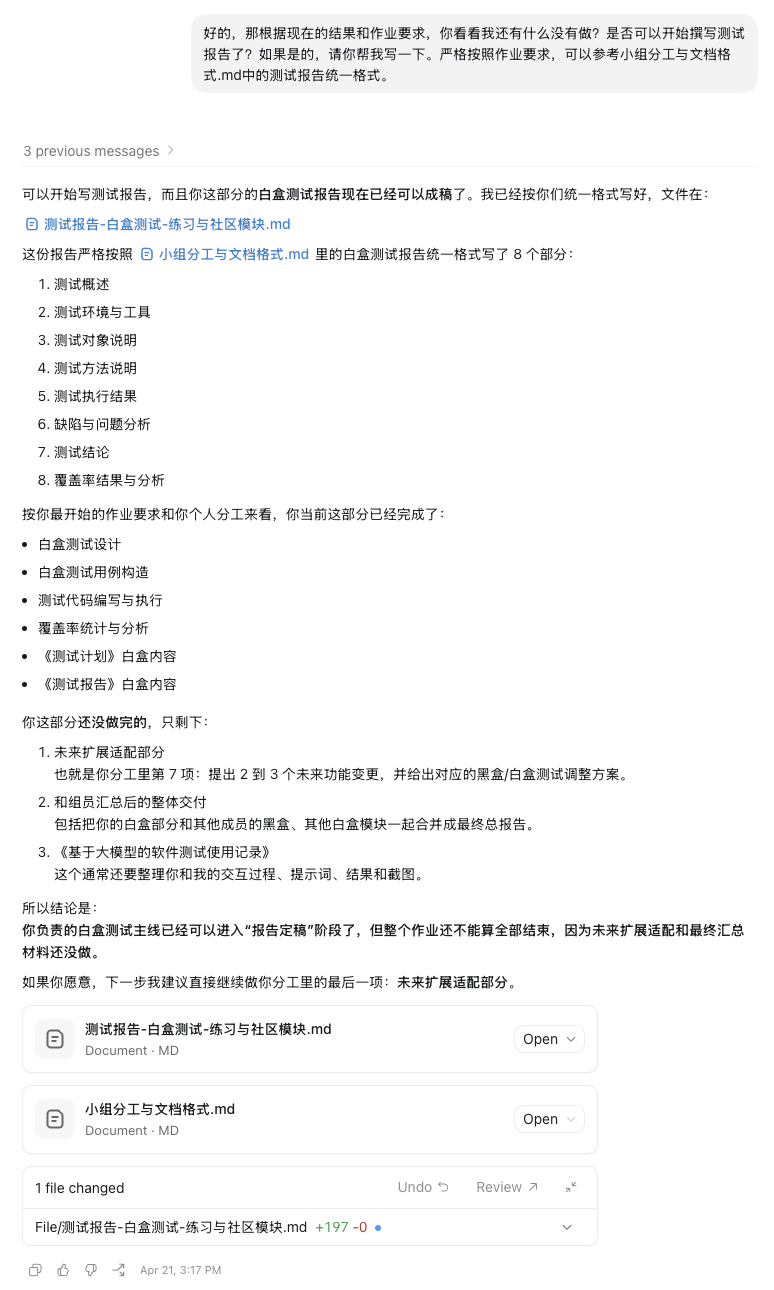
\includegraphics[width=0.82\textwidth]{白盒测试2对话截图/任务5-测试报告-1.png}
  \caption{任务五：按统一模板生成测试报告}
\end{figure}

\begin{figure}[H]
  \centering
  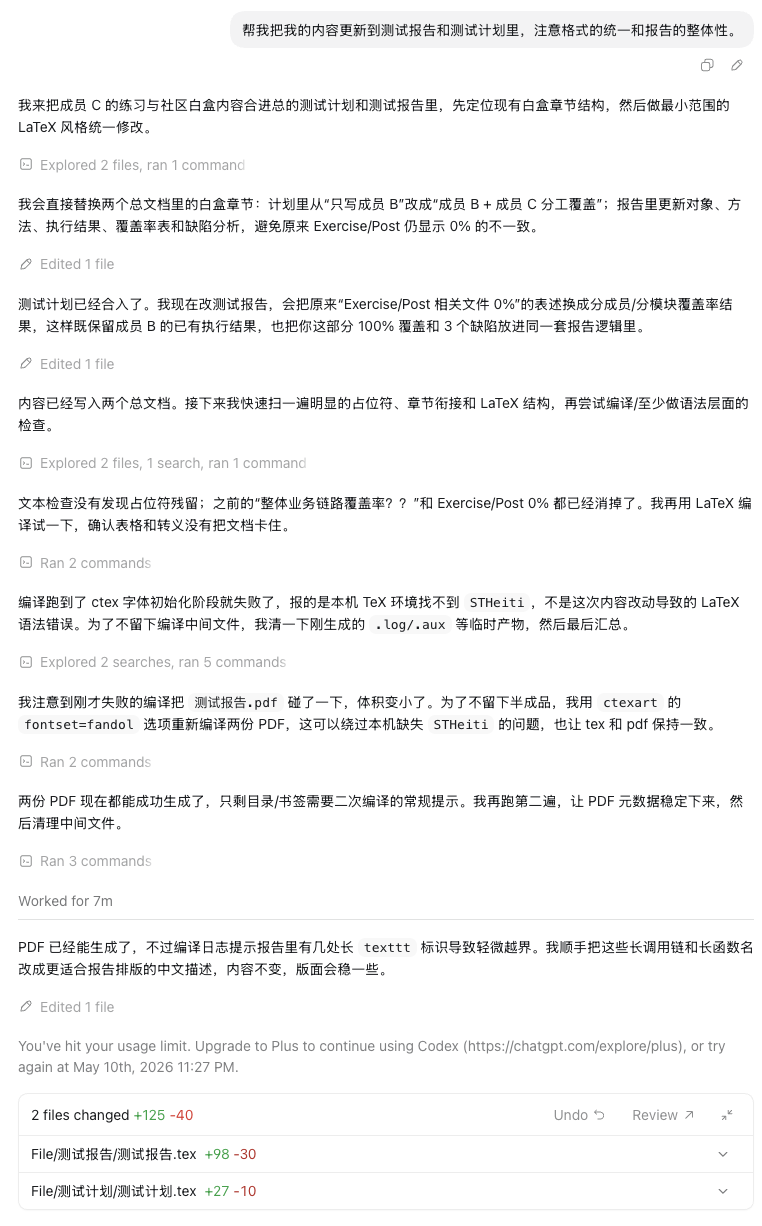
\includegraphics[width=0.82\textwidth]{白盒测试2对话截图/任务5-测试报告-3-合并.png}
  \caption{任务五：将新增内容合并回测试计划与测试报告并统一格式}
\end{figure}

\subsubsection{任务六：未来扩展适配}

由于有 \texttt{failed}，我要求模型补写未来扩展适配。模型围绕练习与社区模块提出 3 项未来变更，并分别给出黑盒/白盒测试调整思路及风险说明。

\begin{figure}[H]
  \centering
  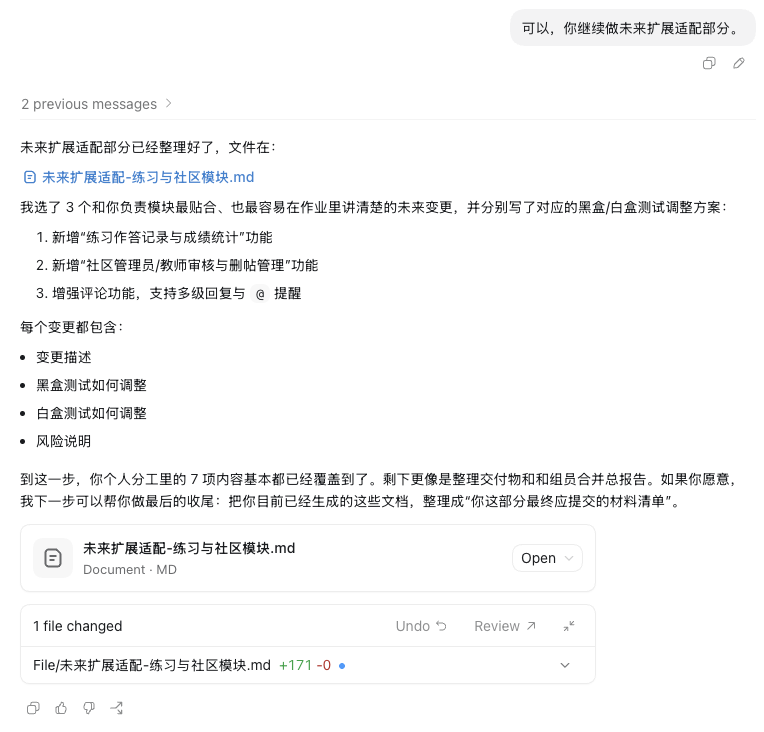
\includegraphics[width=0.82\textwidth]{白盒测试2对话截图/任务6-测试报告-2-未来扩展适配.png}
  \caption{任务六：未来扩展适配与测试调整方案}
\end{figure}

\end{document}
